\documentclass[12pt]{article} 
\usepackage{parskip}    %spaced paragraphs

\usepackage{fancyhdr}
\setlength{\headheight}{30pt}

\usepackage{geometry}   %set margins
\geometry{a4paper, margin=1.5cm}

\usepackage{amsmath}
\usepackage{amssymb}

\usepackage{graphicx}
\graphicspath{ {./figures/} }

\usepackage{fontspec}
\setmainfont{Times New Roman}

\usepackage{siunitx}
\usepackage{steinmetz}  %phasor


\begin{document}

\pagestyle{fancy}
\fancyhead{}
\fancyhead[L]{ES3E6 Assignment}
\fancyhead[R]{1922268}

\section*{Part 1}

\frame{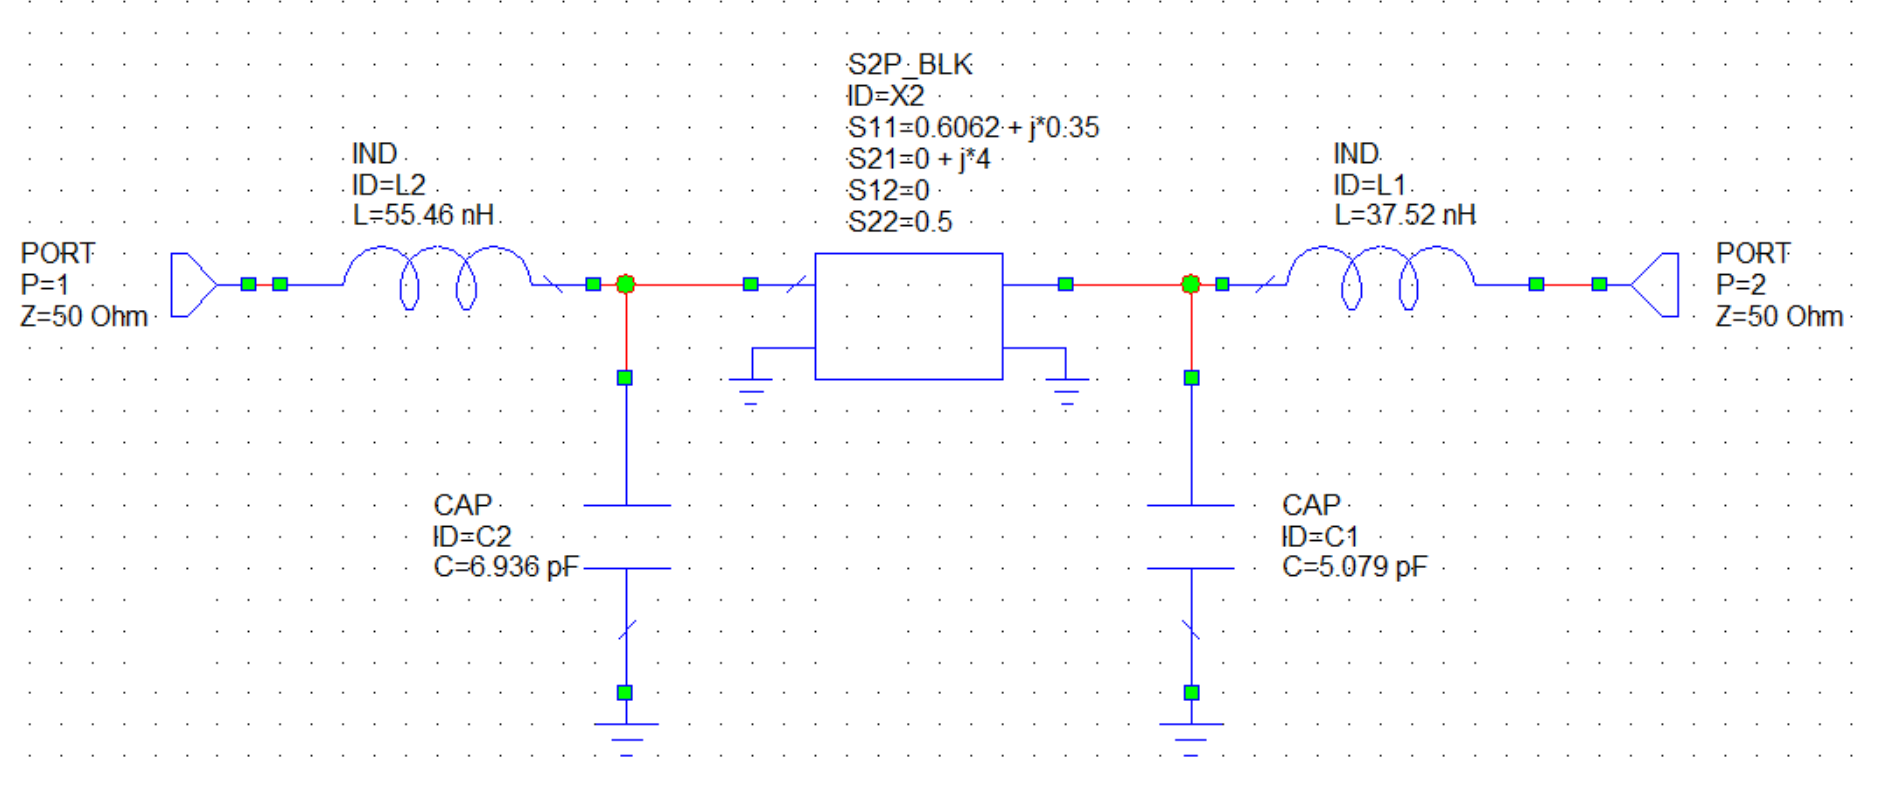
\includegraphics[width=\textwidth]{1 network.png}}
\begin{center}
    \textbf{Matched network.}
\end{center}

\subsection*{(a)}

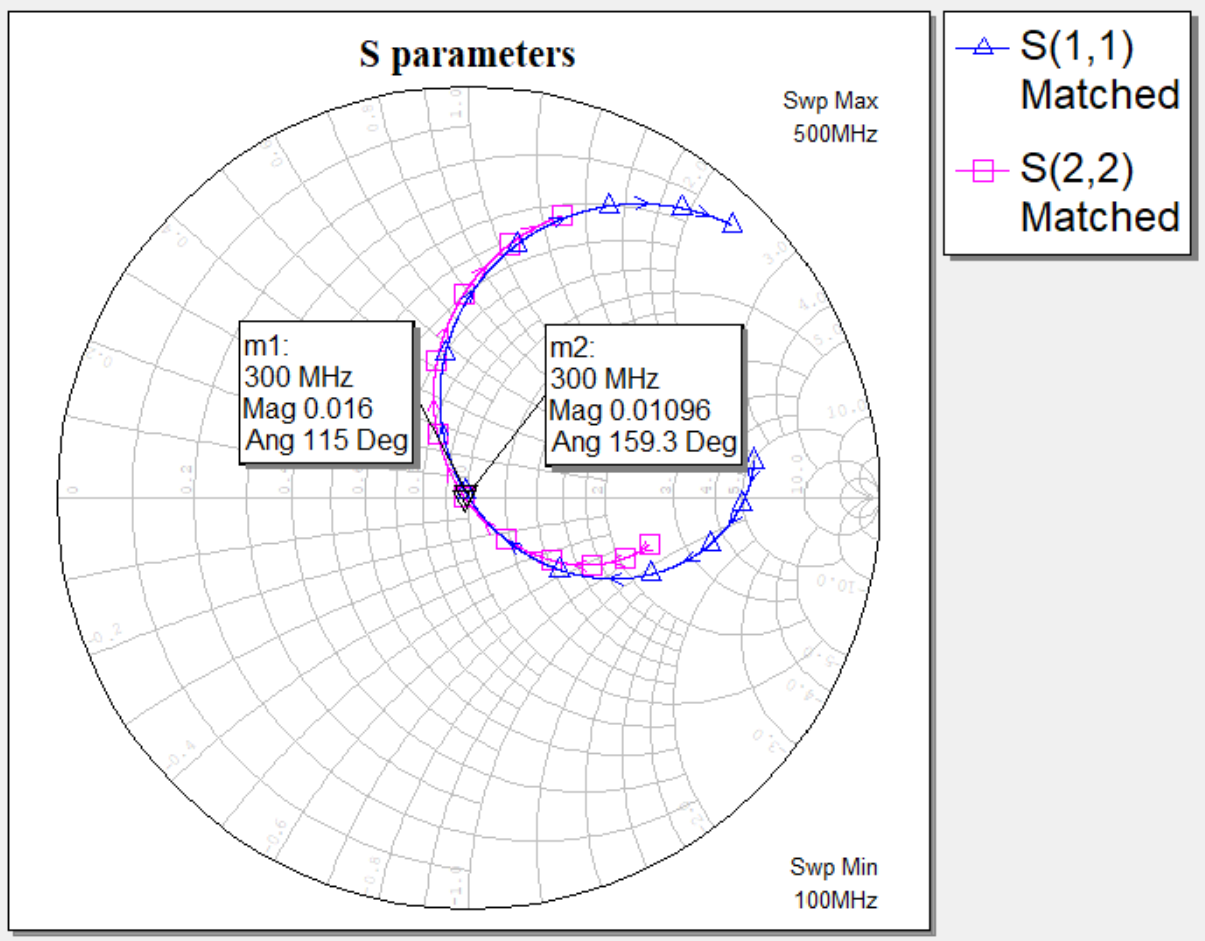
\includegraphics[width=\textwidth]{1 smith chart.png}

The network is matched because, at 300\,\unit{\mega\hertz}, the magnitude of the S\textsubscript{11} and S\textsubscript{22} are very nearly 0.
 
\subsection*{(b)}
\begin{center}
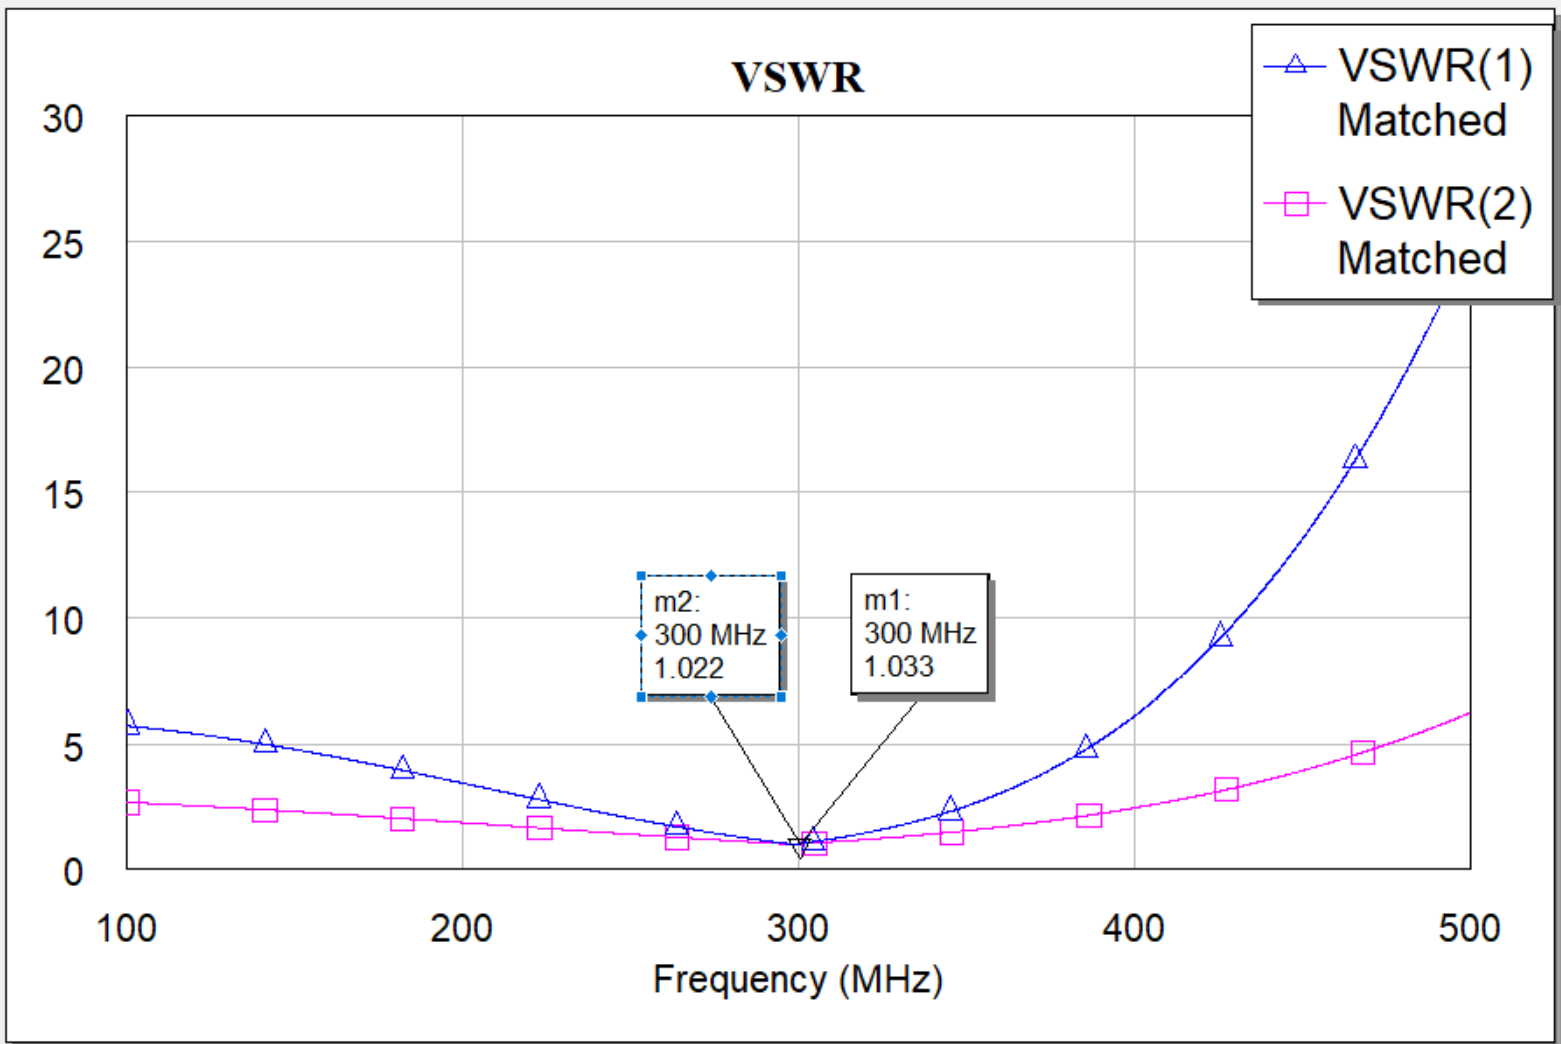
\includegraphics[width=0.8\textwidth]{1 vswr.png}
\end{center}
  
A VSWR of 1 suggests a matched network. At 300\,\unit{\mega\hertz}, the VSWR for the input (1) and output (2) are close to 1.

\subsection*{(c)}
\begin{center}
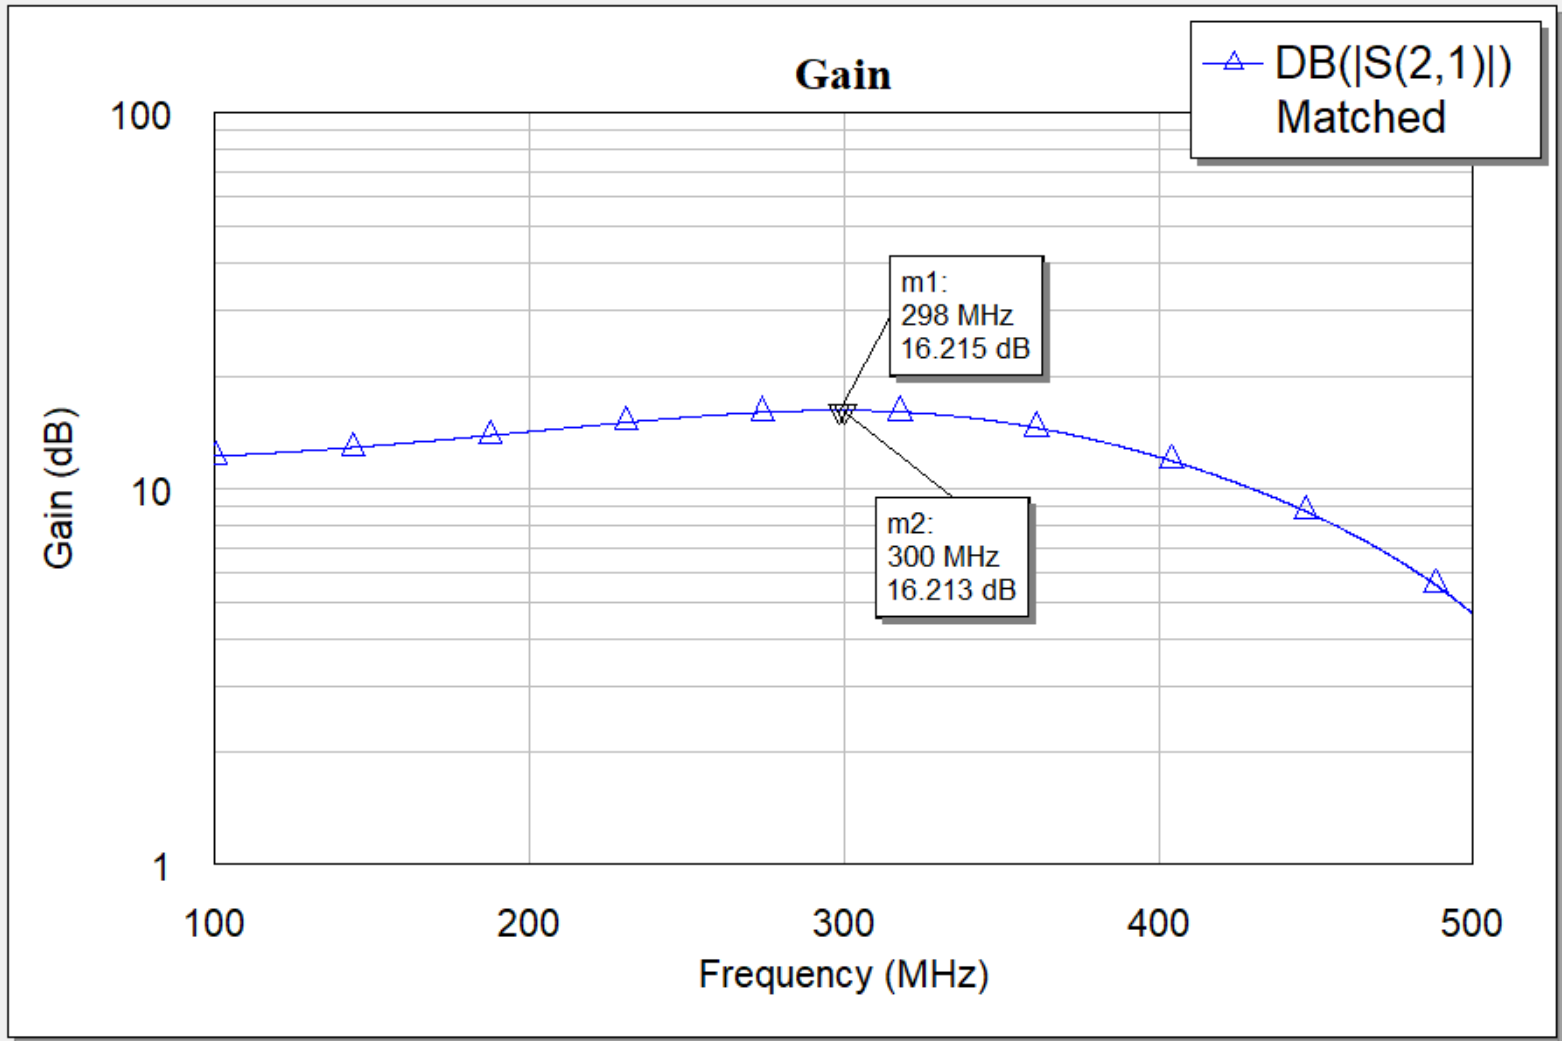
\includegraphics[width=0.8\textwidth]{1 gain.png}
\end{center}

The graph shows the maximum gain (16.215\,\unit{\decibel} at 298\,\unit{\mega\hertz}), and the gain at the frequency designed for (16.213\,\unit{\decibel} at 300\,\unit{\mega\hertz}).
The maximum theoretical gain was calculated to be 16.2149\,\unit{\decibel}.
The gain at the target frequency is very close to this value. 

\subsection*{(d)} 
The following table shows the reflection coefficients and VSWR for the network 
with a source and load impedance of 50\,\unit{\ohm} and +50\% error (75\,\unit{\ohm}) at the source and load.

\begin{center}
\begin{tabular}{|c | c | c | c || c | c | c | c|}
    \hline
    \multicolumn{4}{|c||}{50\,\unit{\ohm} impedance} & \multicolumn{4}{c|}{75\,\unit{\ohm} impedance} \\
    \hline
    |S\textsubscript{11}| & |S\textsubscript{22}| & VSWR\textsubscript{input} & VSWR\textsubscript{output} & |S\textsubscript{11}| & |S\textsubscript{22}| & VSWR\textsubscript{input} & VSWR\textsubscript{output} \\
    \hline
    0.016 & 0.011 & 1.032 & 1.022 & 0.207 & 0.210 & 1.52 & 1.53 \\
    \hline
\end{tabular}
\end{center}


As can be seen, the reflection coefficients and VSWR values increase when the impedance changes,
showing that the network has now become mismatched as they are no longer close to 0 and 1 respectively. 
There is no longer maximum power transfer, however the values are not significantly out of scope,
meaning that the network is still useable, if less efficient.

\section*{Part 2}
\begin{center}
\begin{tabular}{|c|c|}
\hline
\textbf{Parameter} & \textbf{Value} \\
\hline
Centre frequency & 1.9\,\unit{\giga\hertz} \\
I\textsubscript{CQ}& 1\,\unit{\milli\ampere} \\
\textsubscript{CEQ}& 2\,\unit{\volt} \\
Characteristic impedance& 60\,\unit{\ohm} \\
\hline
\end{tabular}

\textbf{Design parameters.}
\end{center}

\subsection*{(a)}

\begin{center}
\begin{tabular}{|c|c|c|c|}
    \hline
    S\textsubscript{11} & S\textsubscript{22} & S\textsubscript{21} & S\textsubscript{12} \\
    \hline  
    $-0.34483 - j0.36677$ & $0.40727 - j0.4538$ & $0.37658 + j1.8228$ & $0.13037 + j0.090698$ \\
    \hline
\end{tabular}

    \textbf{S parameters.}
\end{center}

\subsection*{(b)}

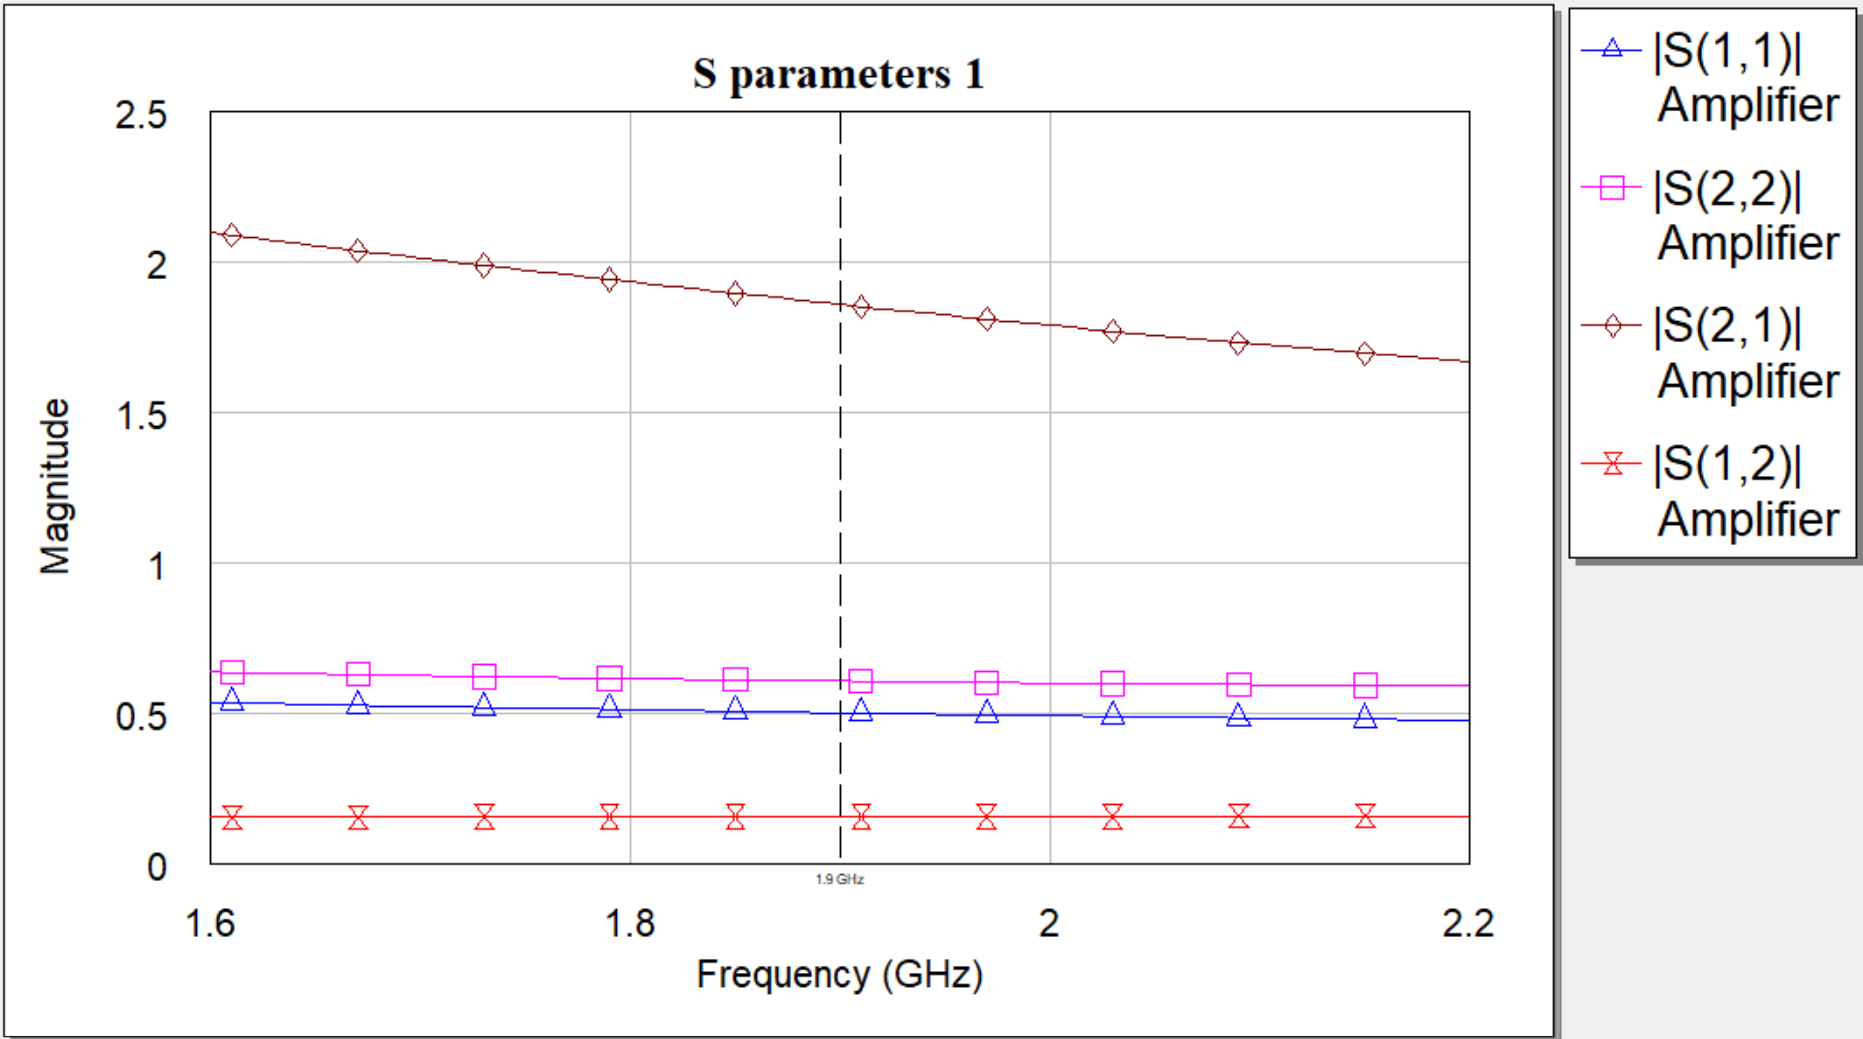
\includegraphics[width=\textwidth]{2 s params.png}

\subsection*{(c)}
\begin{center}
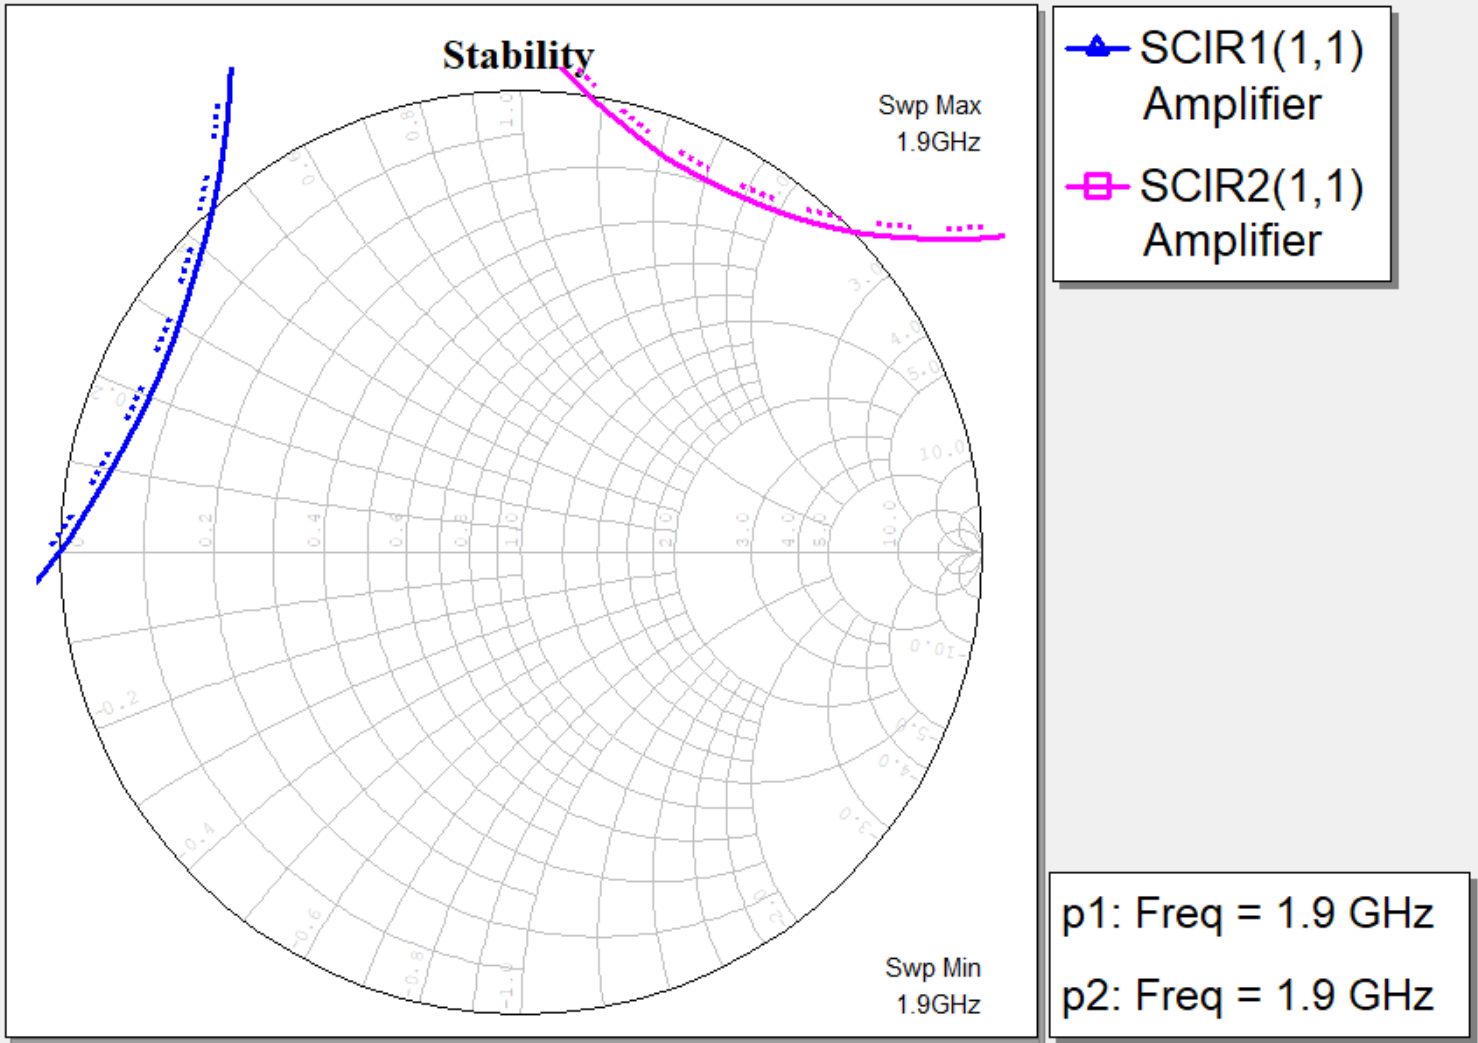
\includegraphics[width=0.9\textwidth]{2 stability.png}
\end{center}

The Smith chart shows shows potential for instability at the given bias point (at 1.9\,\unit{\giga\hertz}). 

The circuit is subsequently modified to include a 434\,\unit{\ohm} stabilising shunt resistor 
and DC-blocking capacitor (Murata GQM1875C2E200GB12 20\,\unit{\pico\farad}).

\begin{center}
    \frame{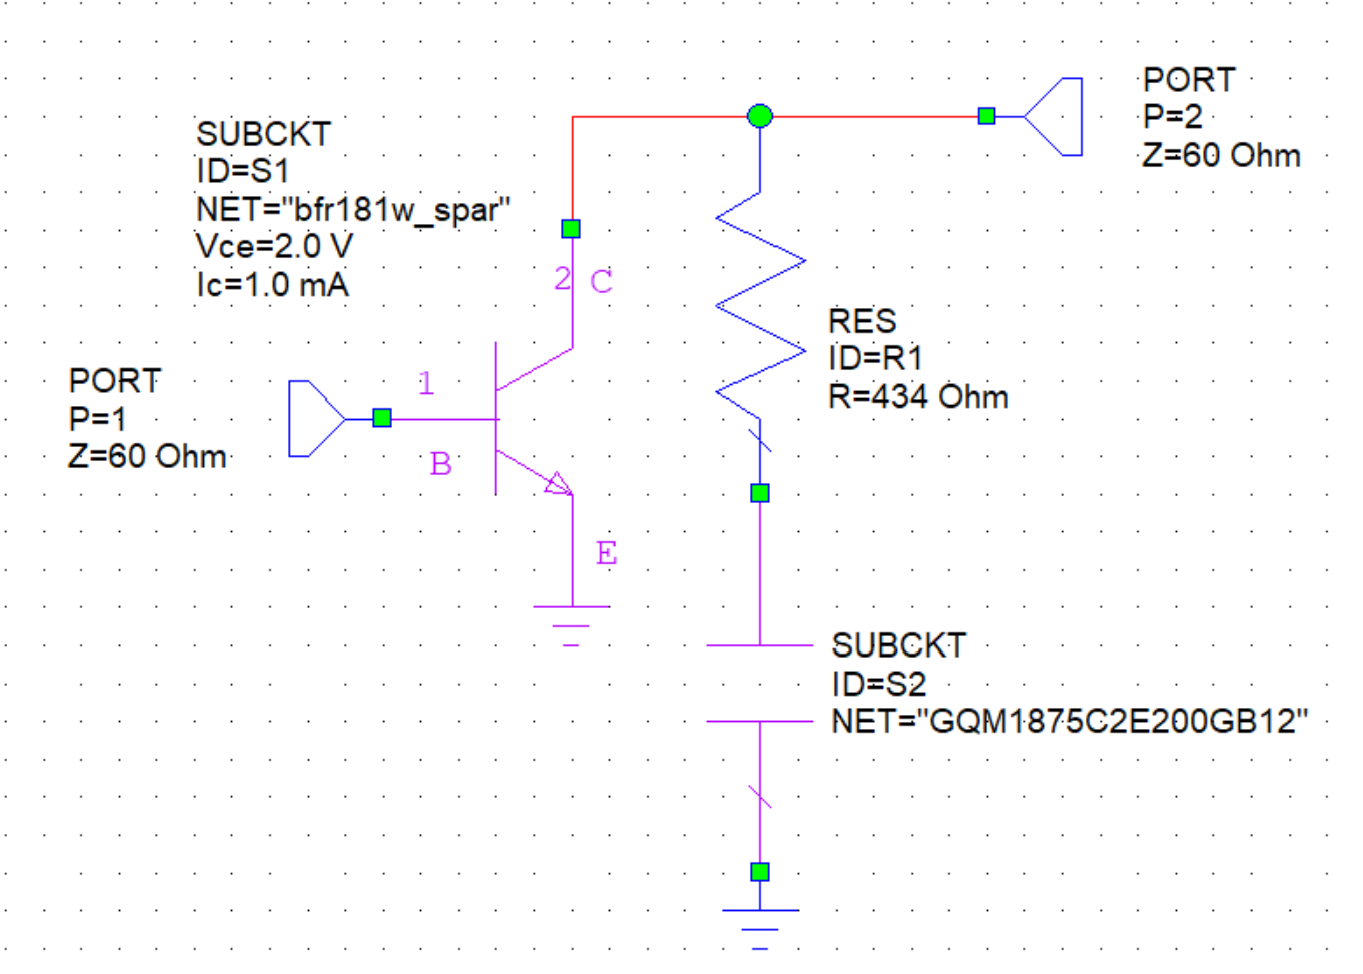
\includegraphics[width=0.9\textwidth]{2 stabilised circuit.png}}
\end{center}

This produces the following stability circles:

\begin{center}
    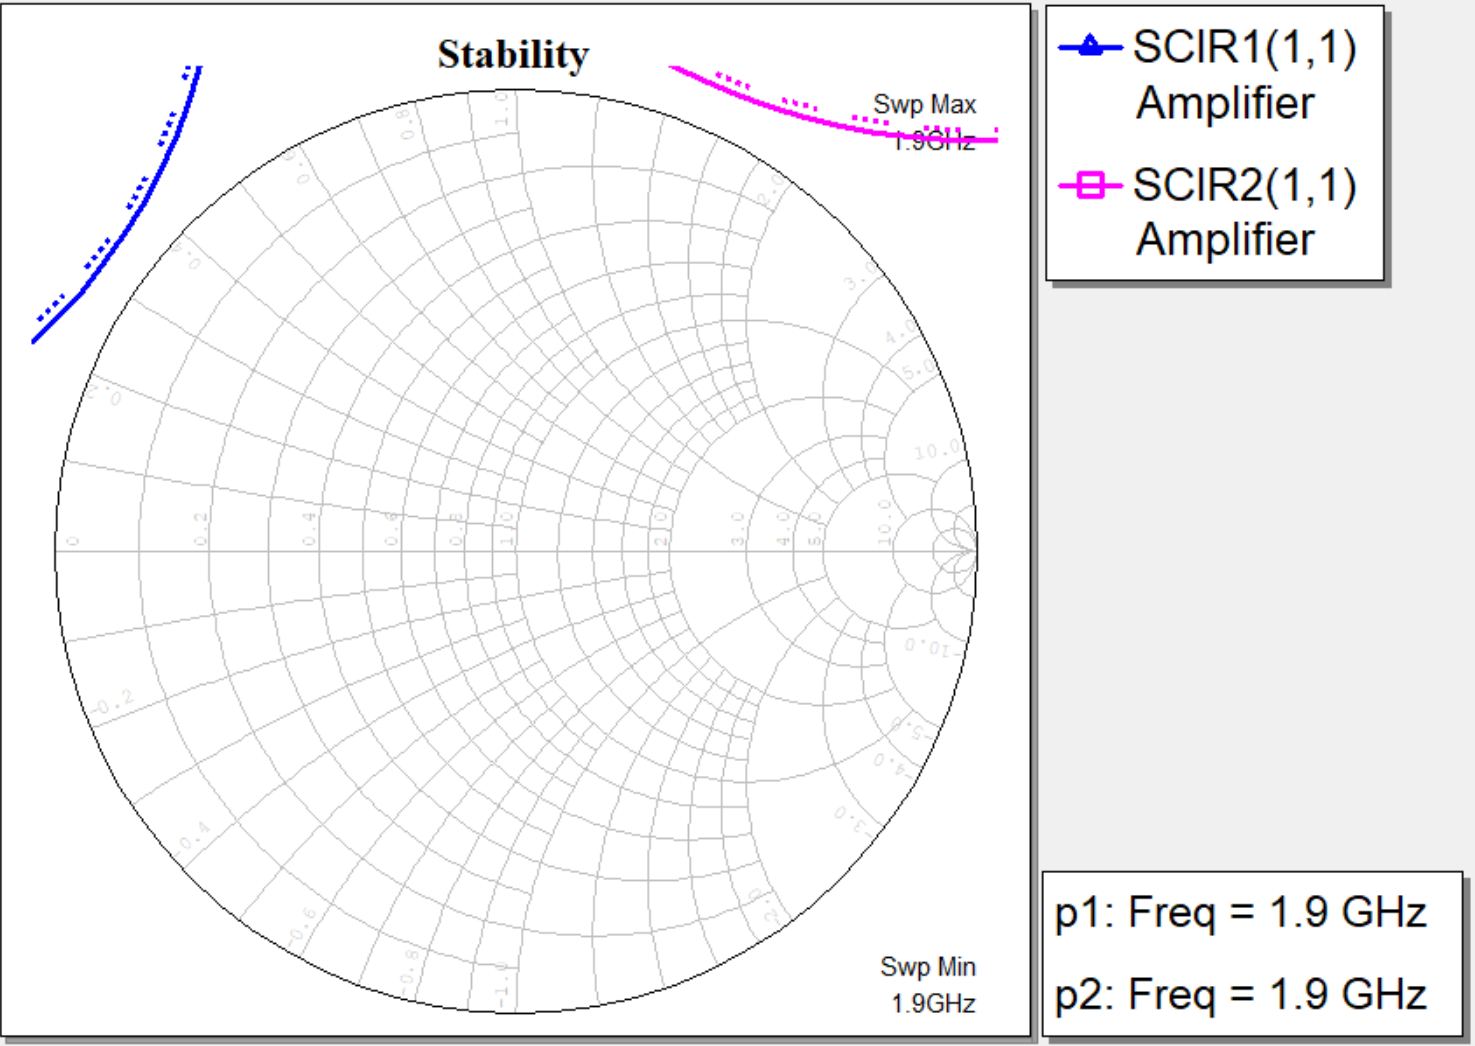
\includegraphics[width=0.9\textwidth]{2 stability 2.png}
\end{center}

As can be seen the circuit is now unconditionally stable at 1.9\,\unit{\giga\hertz} (the stability circles are unreachable).
There is some excessive noise introduction; this can be improved by increasing the resistor size, 
however the current resistor is designed for the overall frequency span ensuring unconditional stability across the 
entire operating frequency range (1.6\,\unit{\giga\hertz} - 2.2\,\unit{\giga\hertz}).

\subsection*{(d)}
The following two graphs are two different types of stability measures. The circuit is unconditionally stable across the operating range
as no stability factor drops below 1. The graphs have markers to indicate the minimum value of stability found.

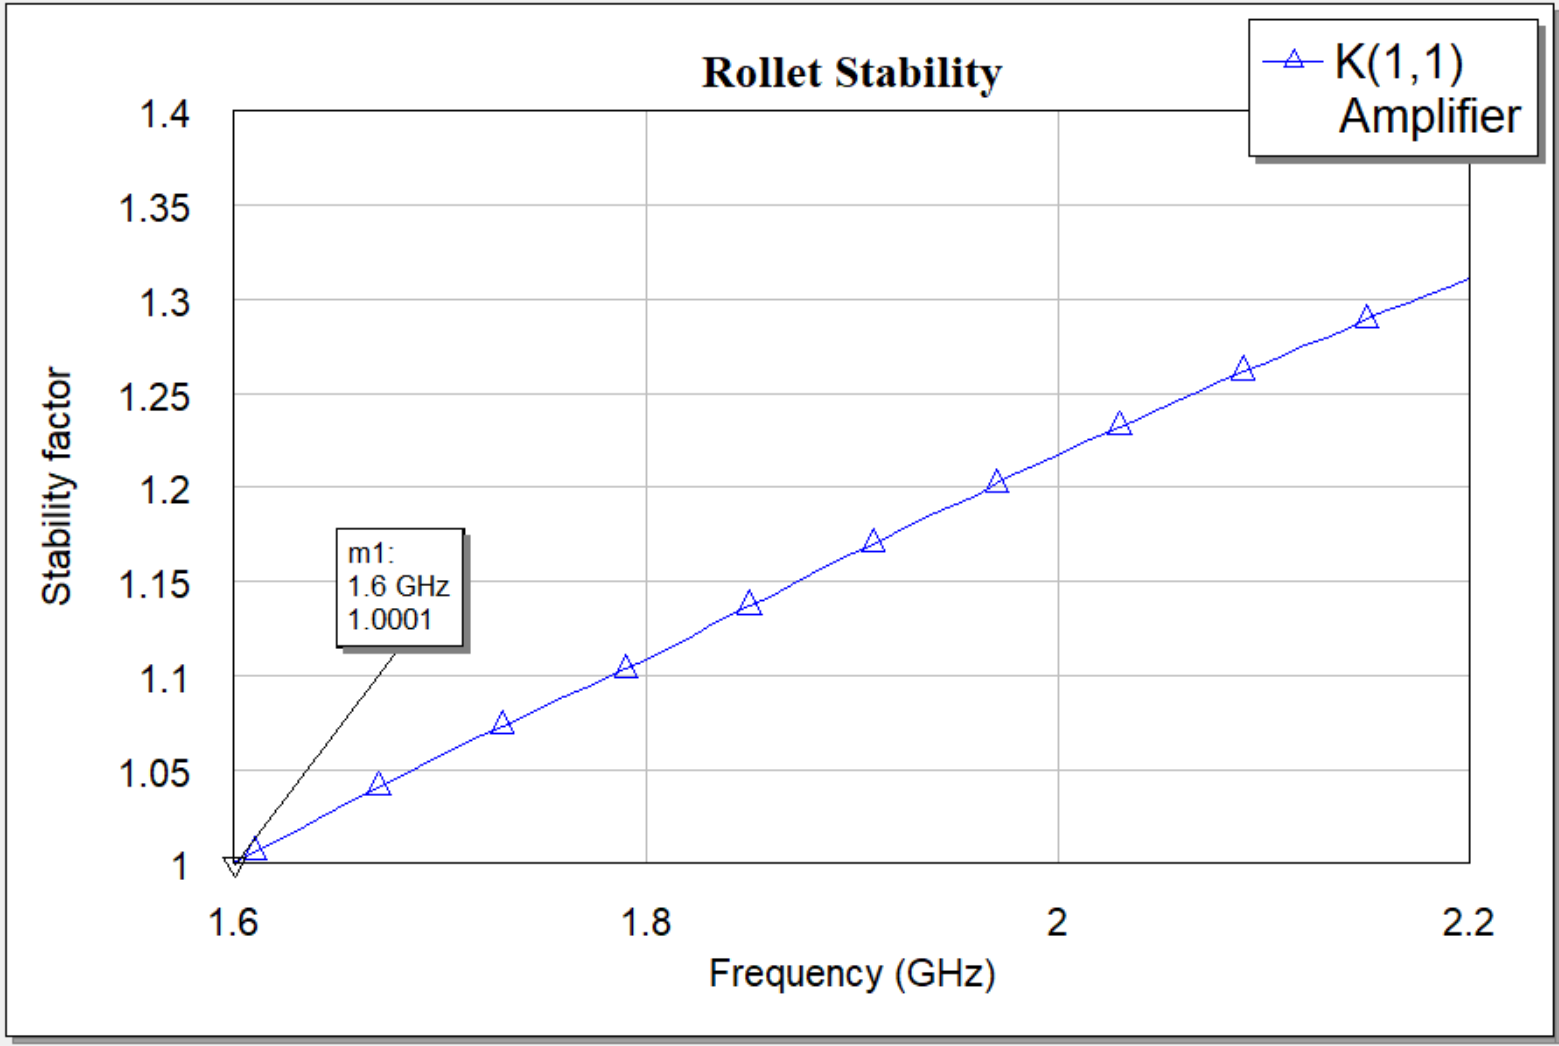
\includegraphics[width=\textwidth]{2 rollet stability.png}

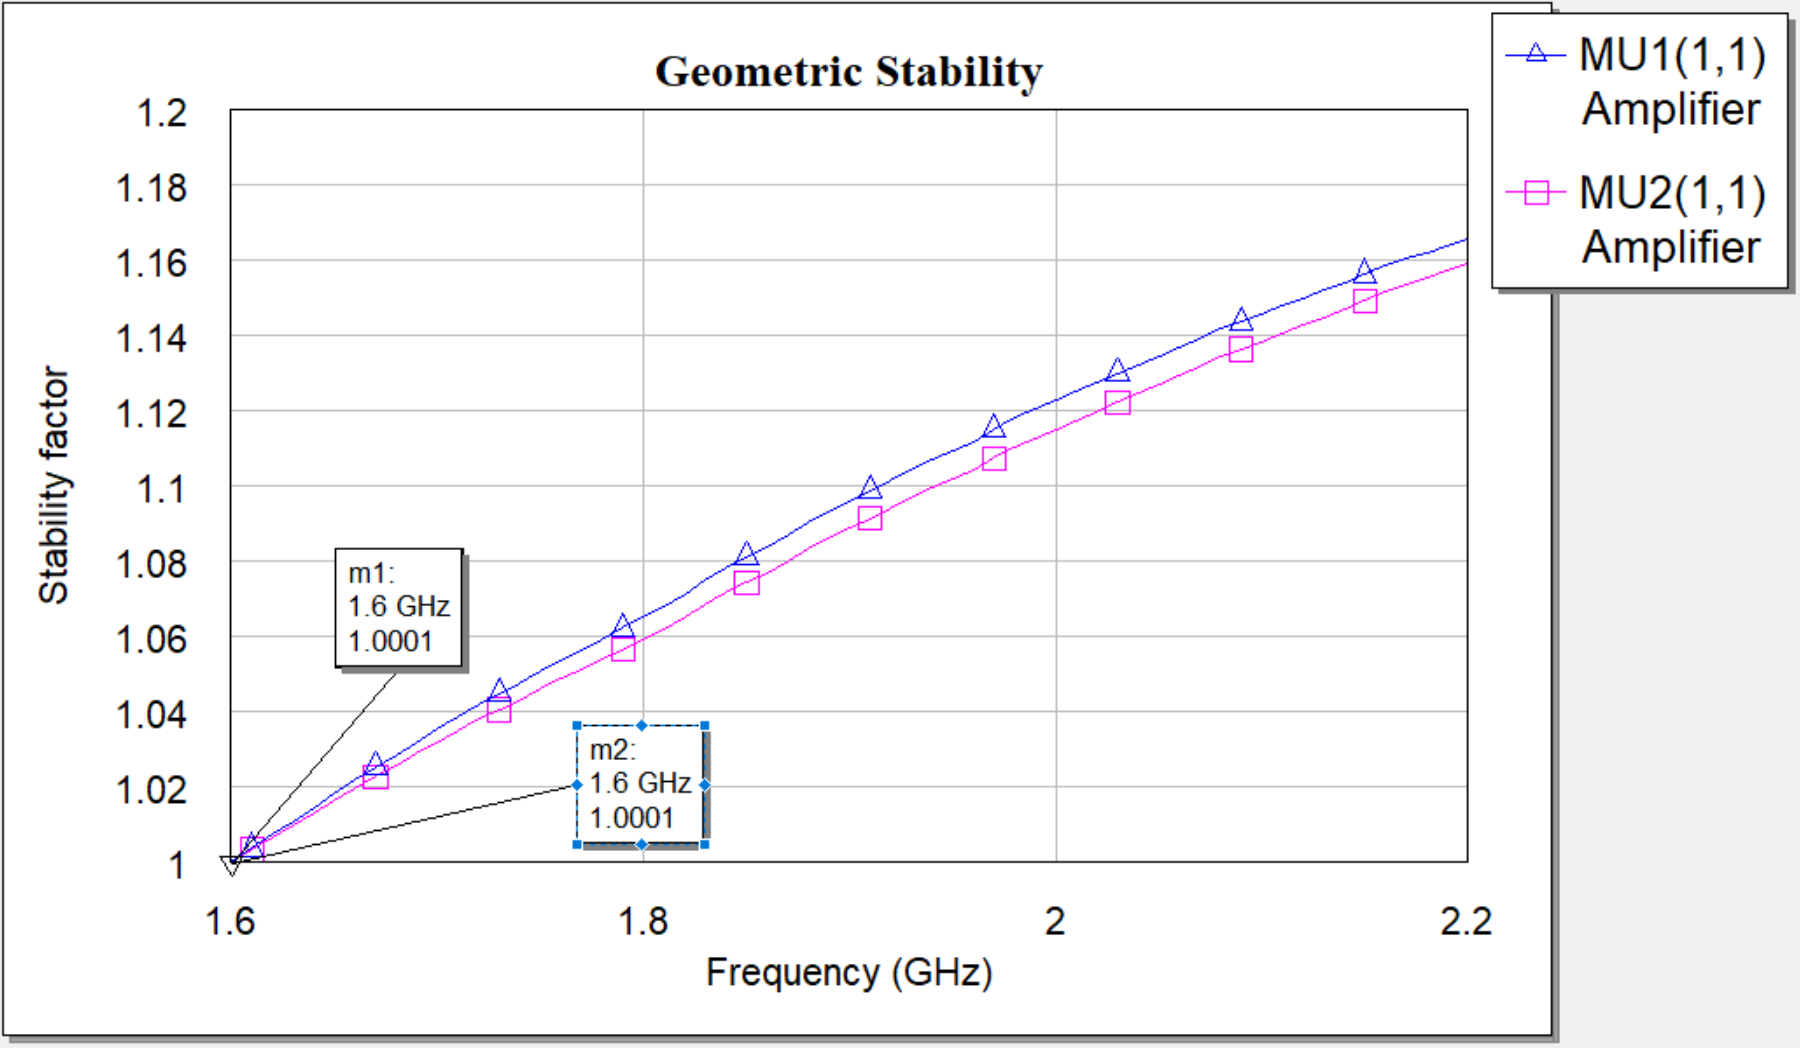
\includegraphics[width=\textwidth]{2 geometric stability.png}

\section*{Part 3}
\subsection*{(a)}

$\Gamma_S = -0.5926 + j0.4313, \quad \Gamma_L = 0.2822 + j0.6573$

Therefore:

$Z_S = 10.2015 + j19.0097, \quad Z_L = 30.9293 + j83.2718$

\begin{center}
\frame{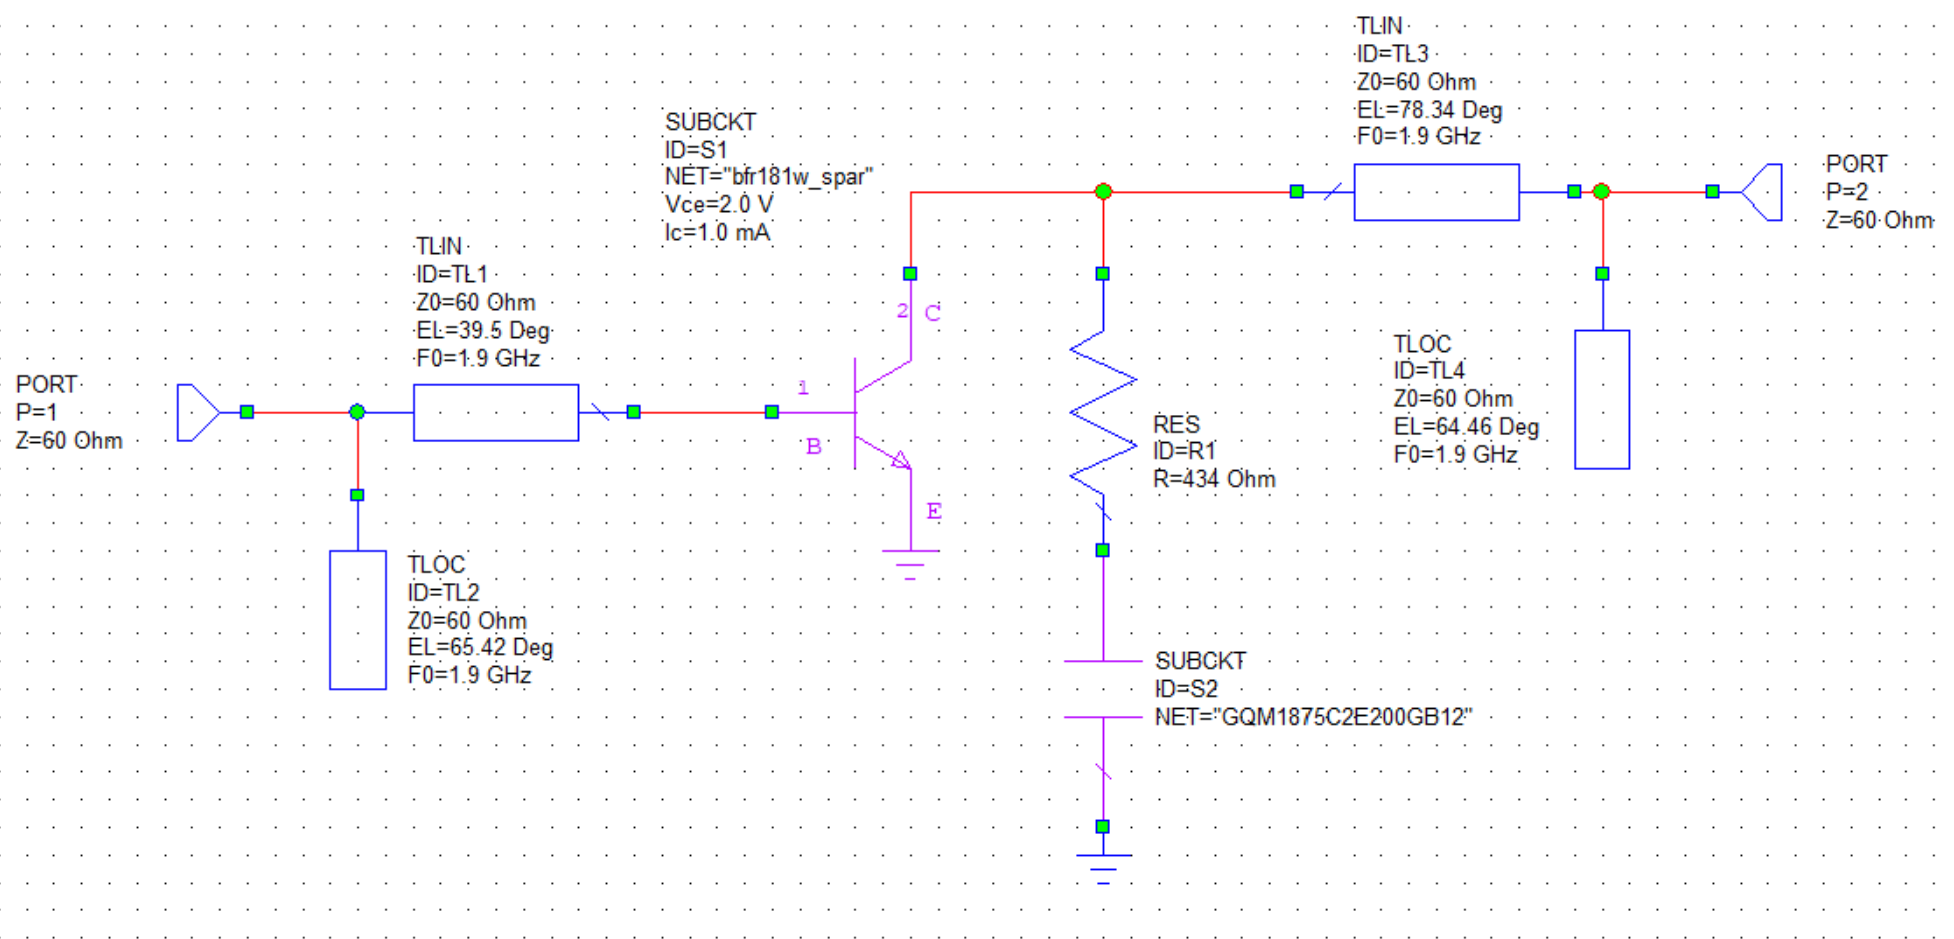
\includegraphics[width=\textwidth]{3 matched network.png}}
\textbf{Simultaneous conjugate matched circuit.}
\end{center}

\subsection*{(b)}

\begin{center}
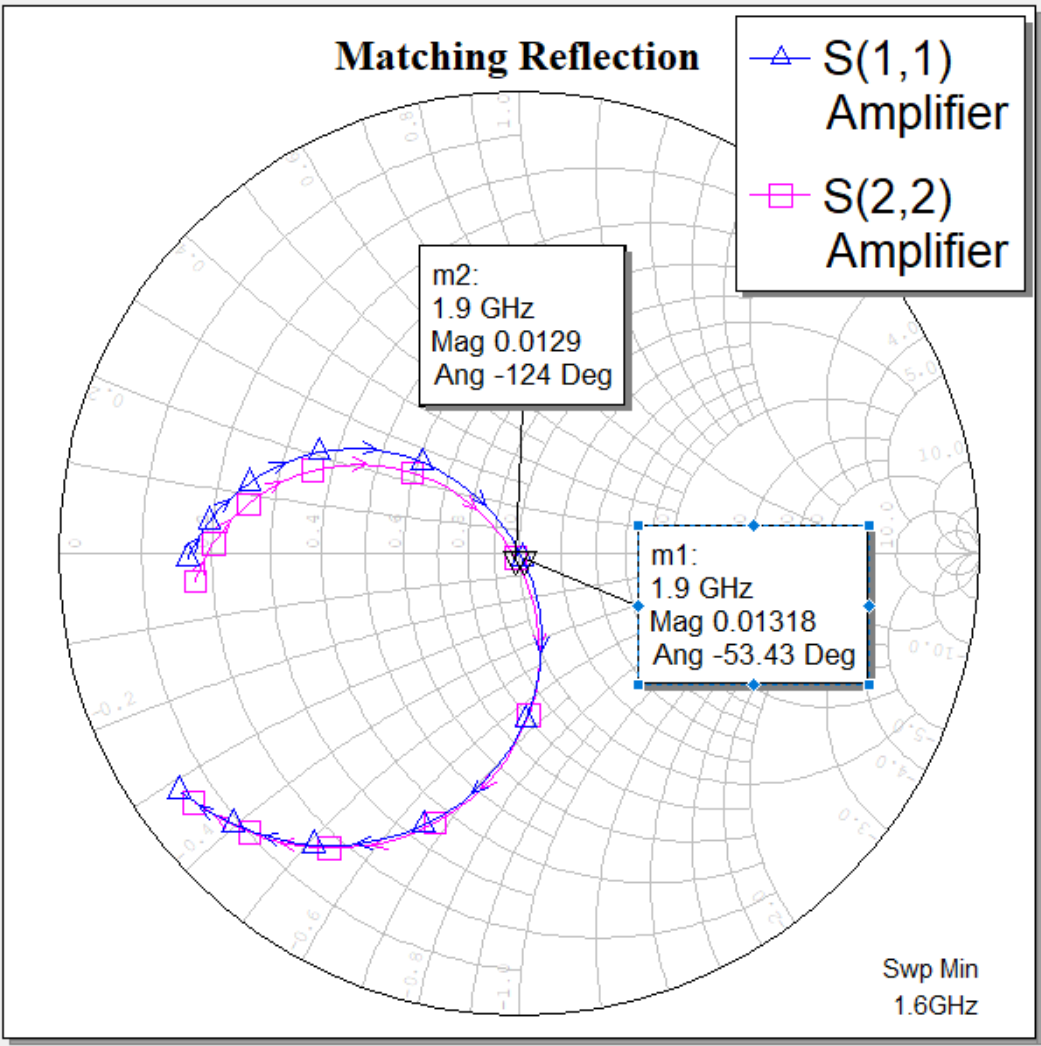
\includegraphics[width=0.8\textwidth]{3 s params.png}
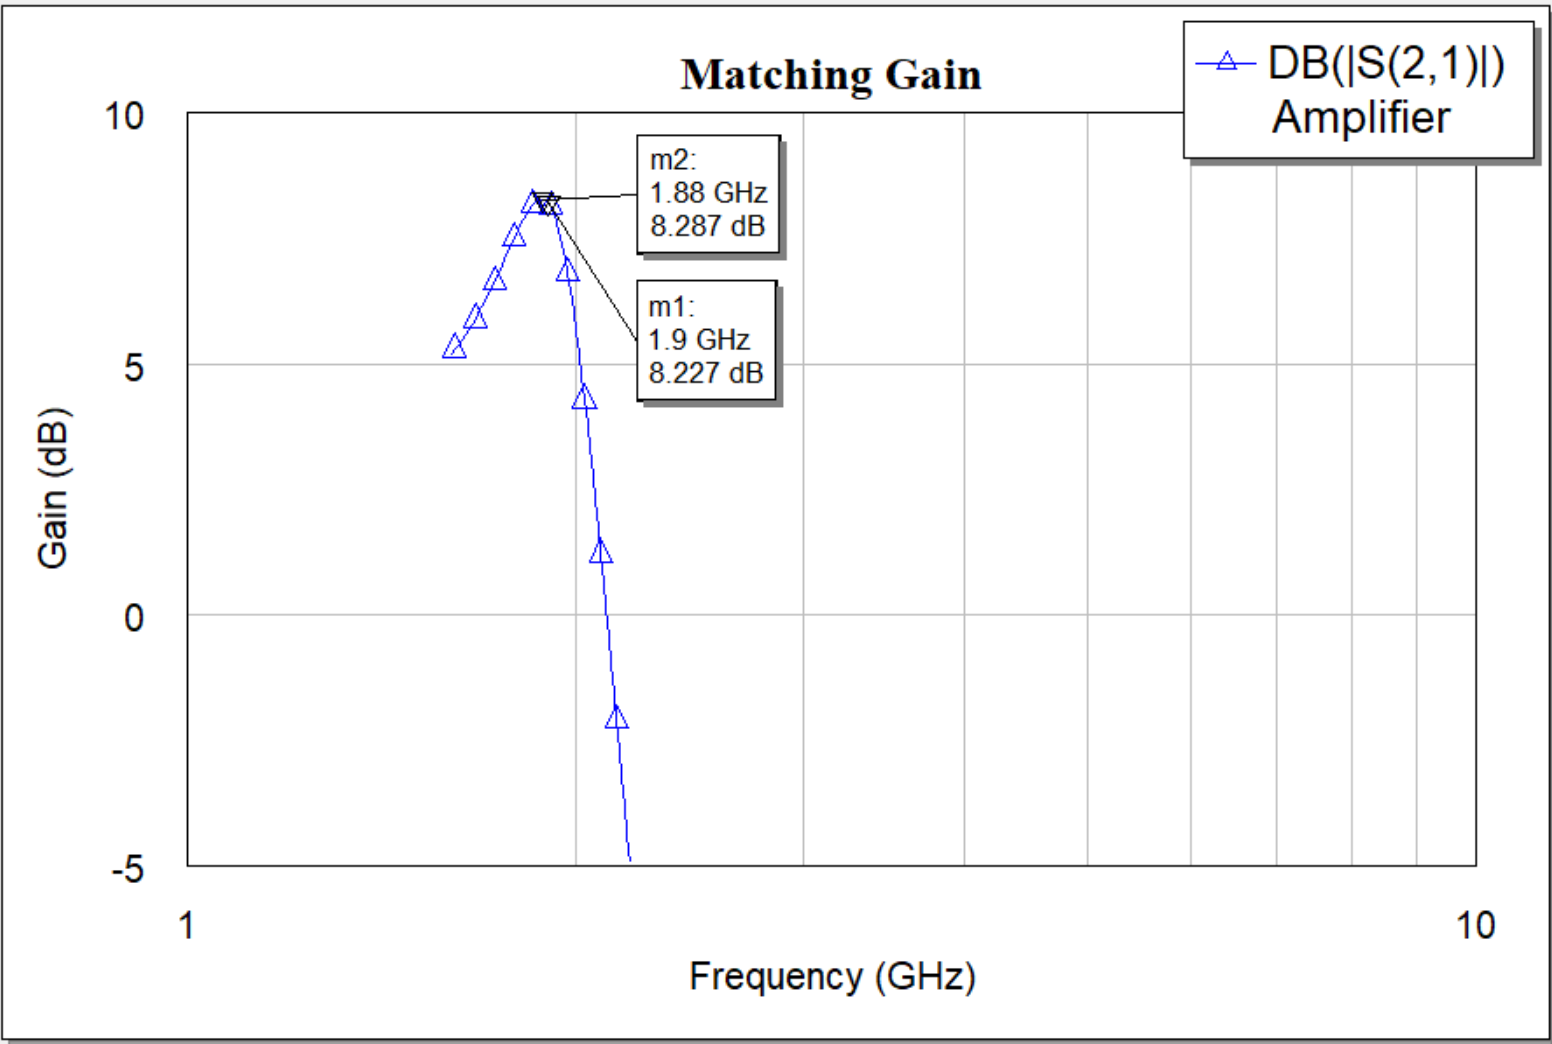
\includegraphics[width=0.8\textwidth]{3 gain.png}
\end{center}
\subsection*{(c)}
The Smith chart shows that, at 1.9\,\unit{\giga\hertz} (the target centre frequency), the S parameters are very close to 0, 
suggesting the system is matched.  

\subsection*{(d)}
The overall performance of the amplifier appears to be good due to matched S parameters and agreement between the theoretical 
and designed gain.

The calculated theoretical maximum gain at 1.9\,\unit{\giga\hertz} is 8.2310\,\unit{\decibel}. The designed gain (8.227\,\unit{\decibel}) reaches this to three significant figures, 
as can be seen on the 1.9\,\unit{\giga\hertz} marker of the Matching Gain chart. 

\section*{Part 4}

\begin{center}
\frame{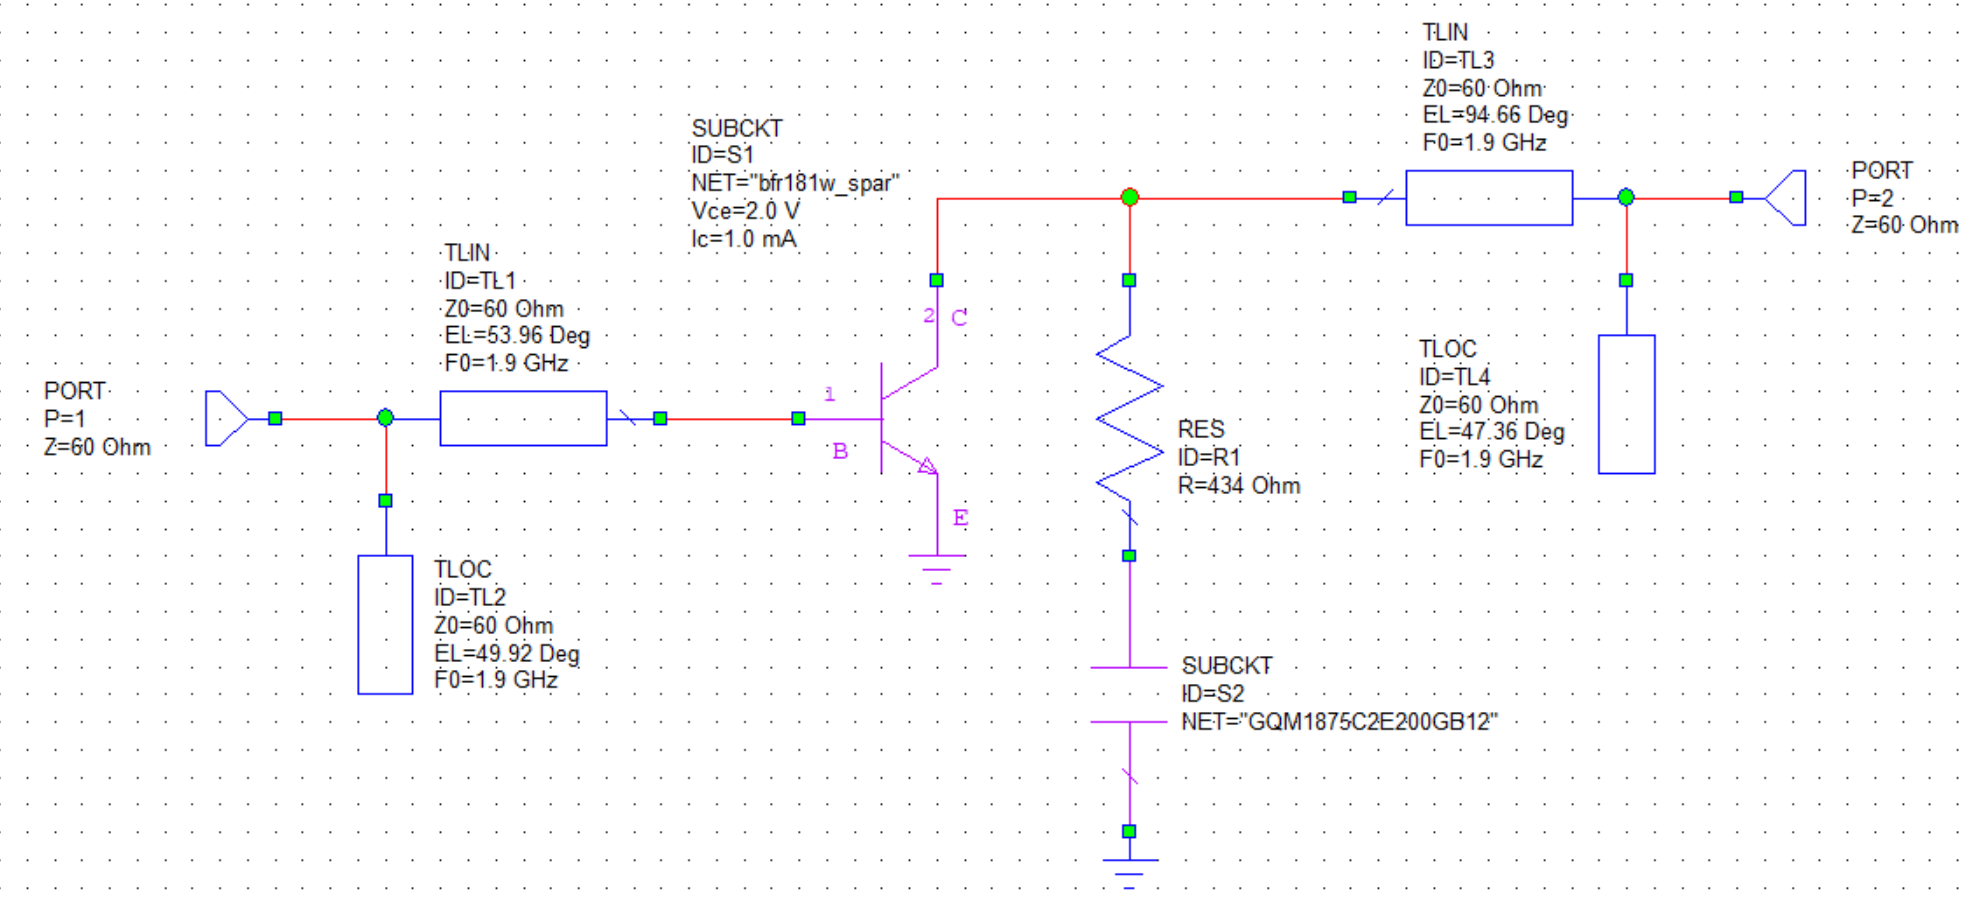
\includegraphics[width=\textwidth]{4 network.png}}

\textbf{Unilateral approximate matched circuit.}  
\end{center}

The following two graphs show the reflection S parameters and gain of the amplifier using the unilateral approximation. 



\begin{center}
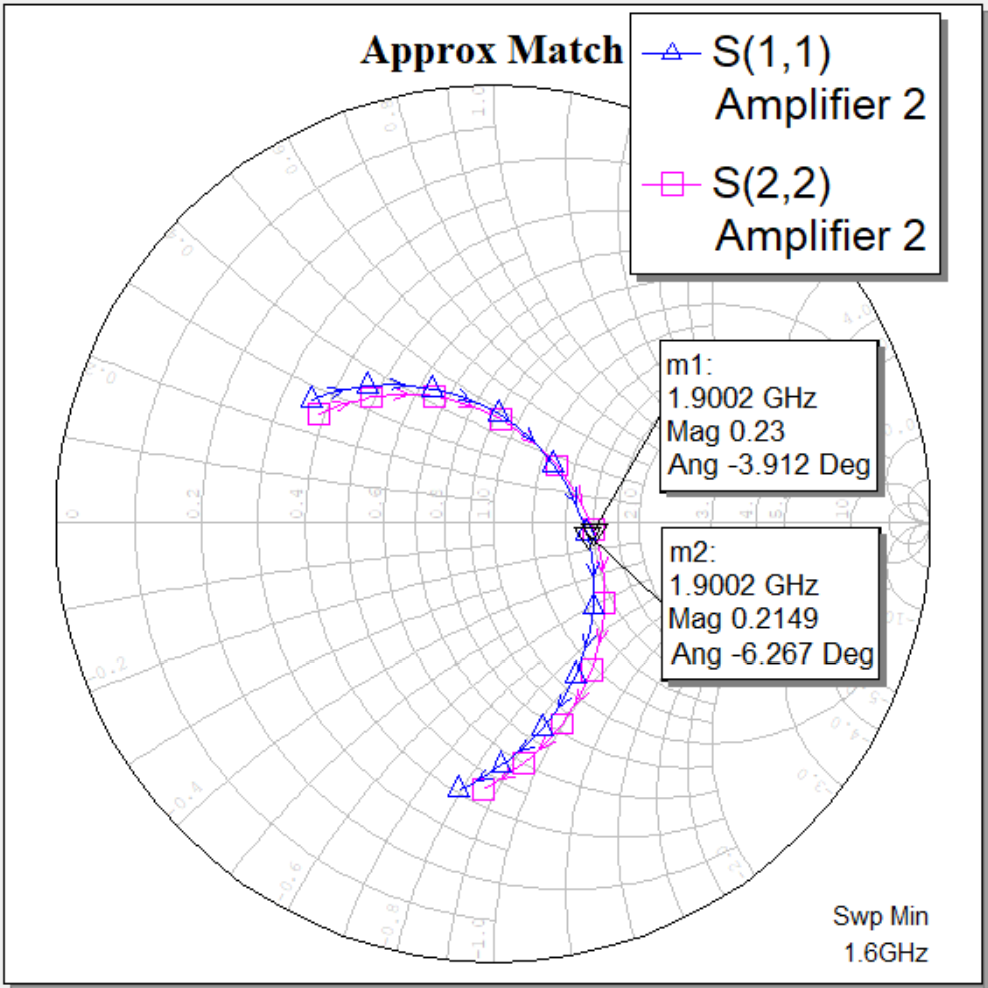
\includegraphics[width=0.8\textwidth]{4 match.png}
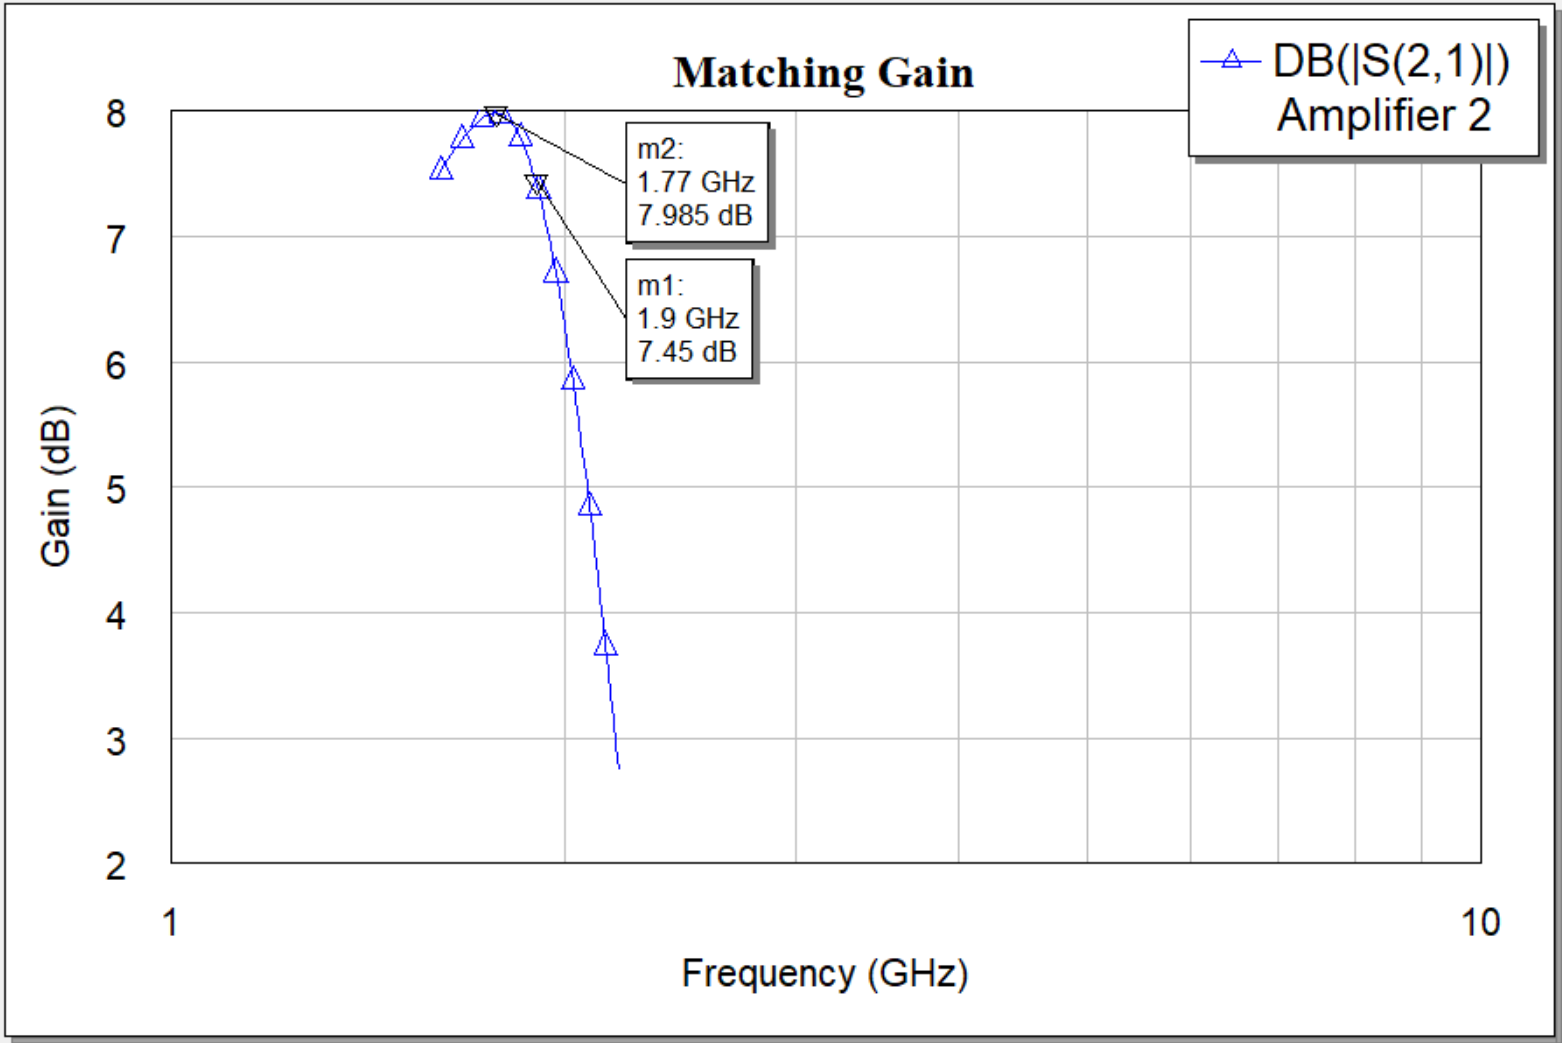
\includegraphics[width=0.8\textwidth]{4 gain.png}
\end{center}

As can be seen, the match is close, but not as good as the simultaneous conjugate match. 
There is greater power reflected than under the simultaneous conjugate match, however overall it is still low.

The gain also suffers and has reduced, with the peak having moved to a lower frequency. 

The unilateral approximation makes amplifier design much simpler, especially as it involves fewer steps. 
However, it relies on $S_{12} = 0$, or at least very small that it can be neglected. 
This network in particular has $\lvert S_{12}\lvert = 0.14$, which is too large to effectively approximate away.
This leads to the designed amplifer performance to be noticeably worse. 

The simultaneous conjugate match produces a network close to the theoretical limits, 
meaning the circuit is almost as good as is possible. However, there are still some estimation and approximation errors
introduced during the design process, which lead the circuit to be very slightly off the theoretical maximums. 
This can be refined with more time spent ensuring precision in the design, however requires ever more time investment with diminishing returns.


\section*{Part 5}
\subsection*{(a)}


\begin{center}
    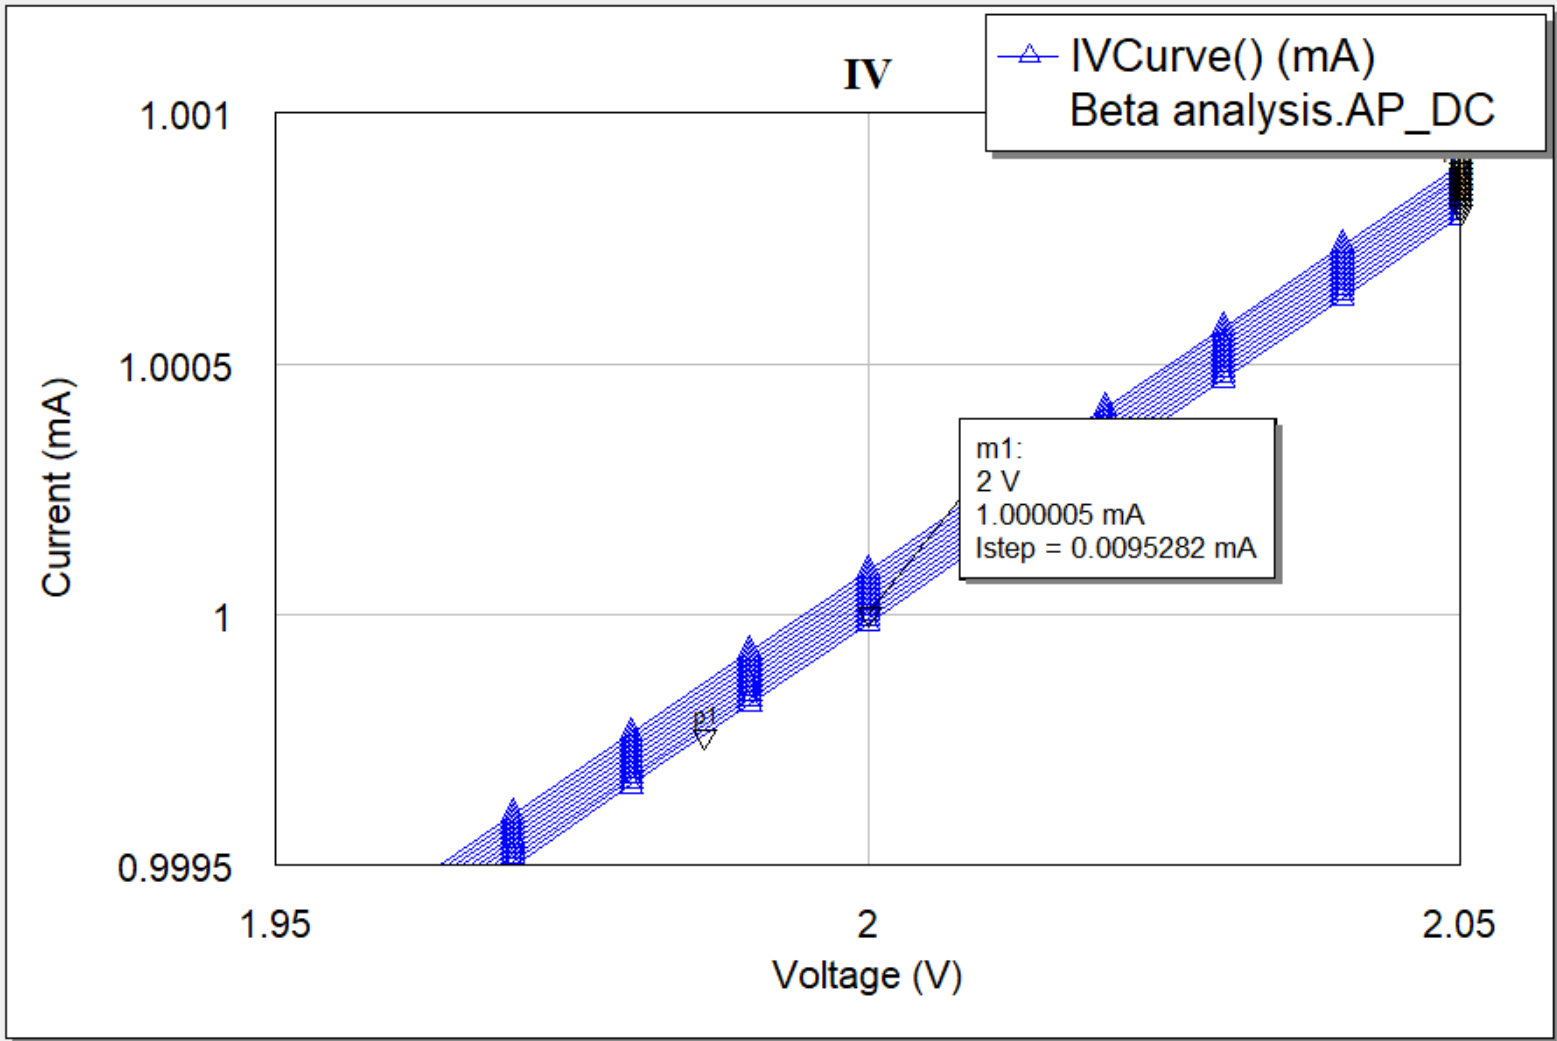
\includegraphics[width=\textwidth]{5 iv.png}

    \textbf{IV curve trace of BFR181W transistor.}
\end{center}
The graph shows that $ I_C \cong 1\,\unit{\milli\ampere} $ when $ I_B = 0.0095282\,\unit{\milli\ampere} $. $ I_C = \beta I_B \Rightarrow \beta = 104.952$.

\subsection*{(b)}

$ V_C = V_{CC} - R_C (I_C + I_B) \Rightarrow R_C = 1981.113\,\unit{\ohm}$. For simplicity and reduced noise (theoretically)
a single resistor will be used. The closest E192 is 1.98\,\unit{\kilo\ohm}.

$I_B = \frac{V_C - V_B}{R_B} \Rightarrow R_B \simeq 137\,\unit{\kilo\ohm}$

\begin{center}
    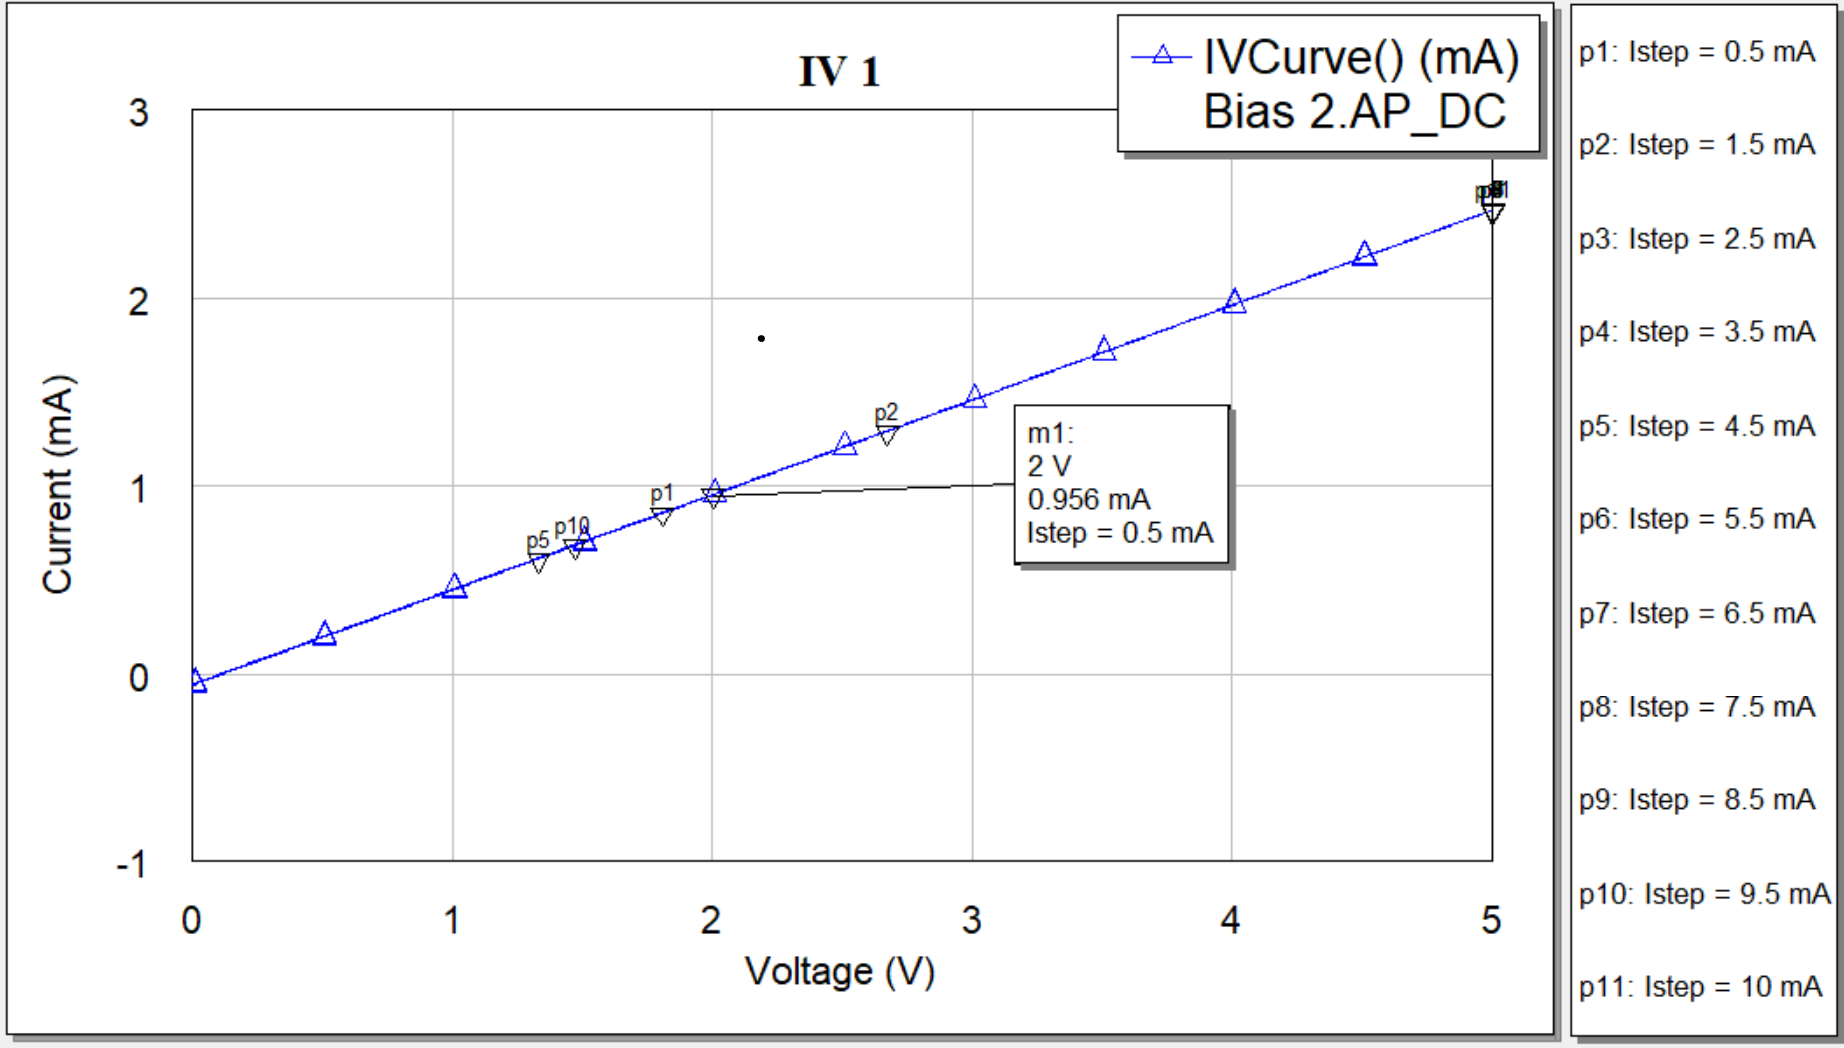
\includegraphics[width=0.9\textwidth]{5 iv1.png}

    \textbf{IV curve of biased transistor, showing stability across current sweep.}
\end{center}

\subsection*{(c)}

\begin{center}
    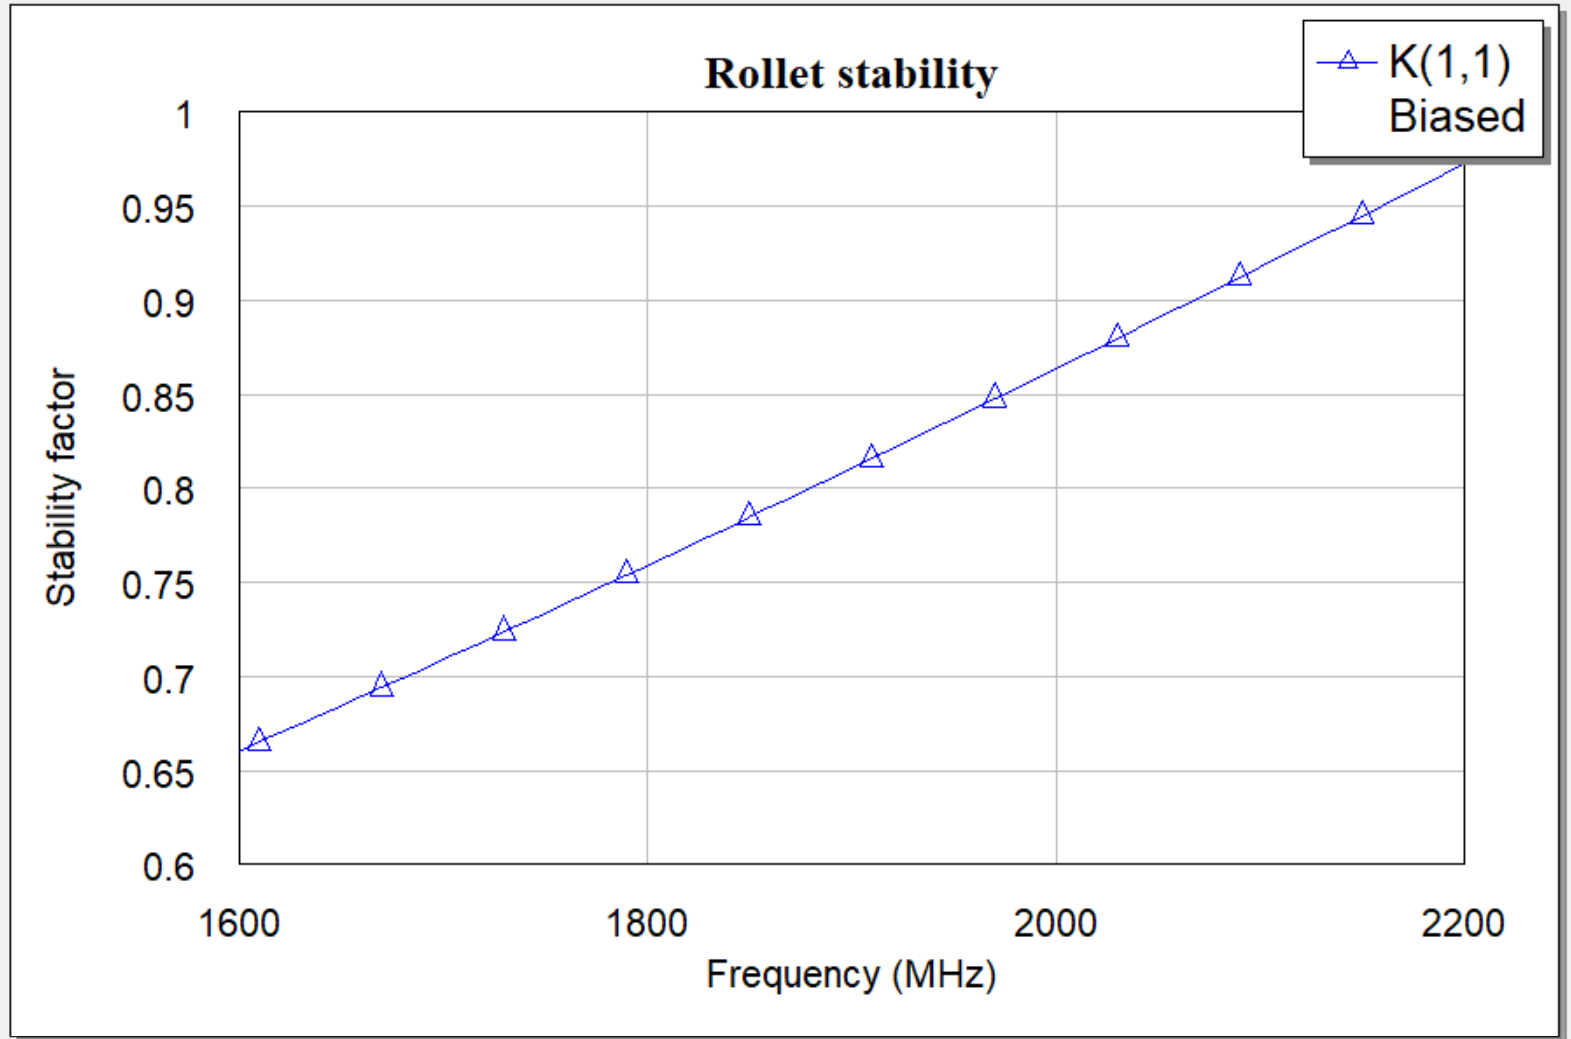
\includegraphics[width=0.5\textwidth]{5 rollet.png}
    \quad
    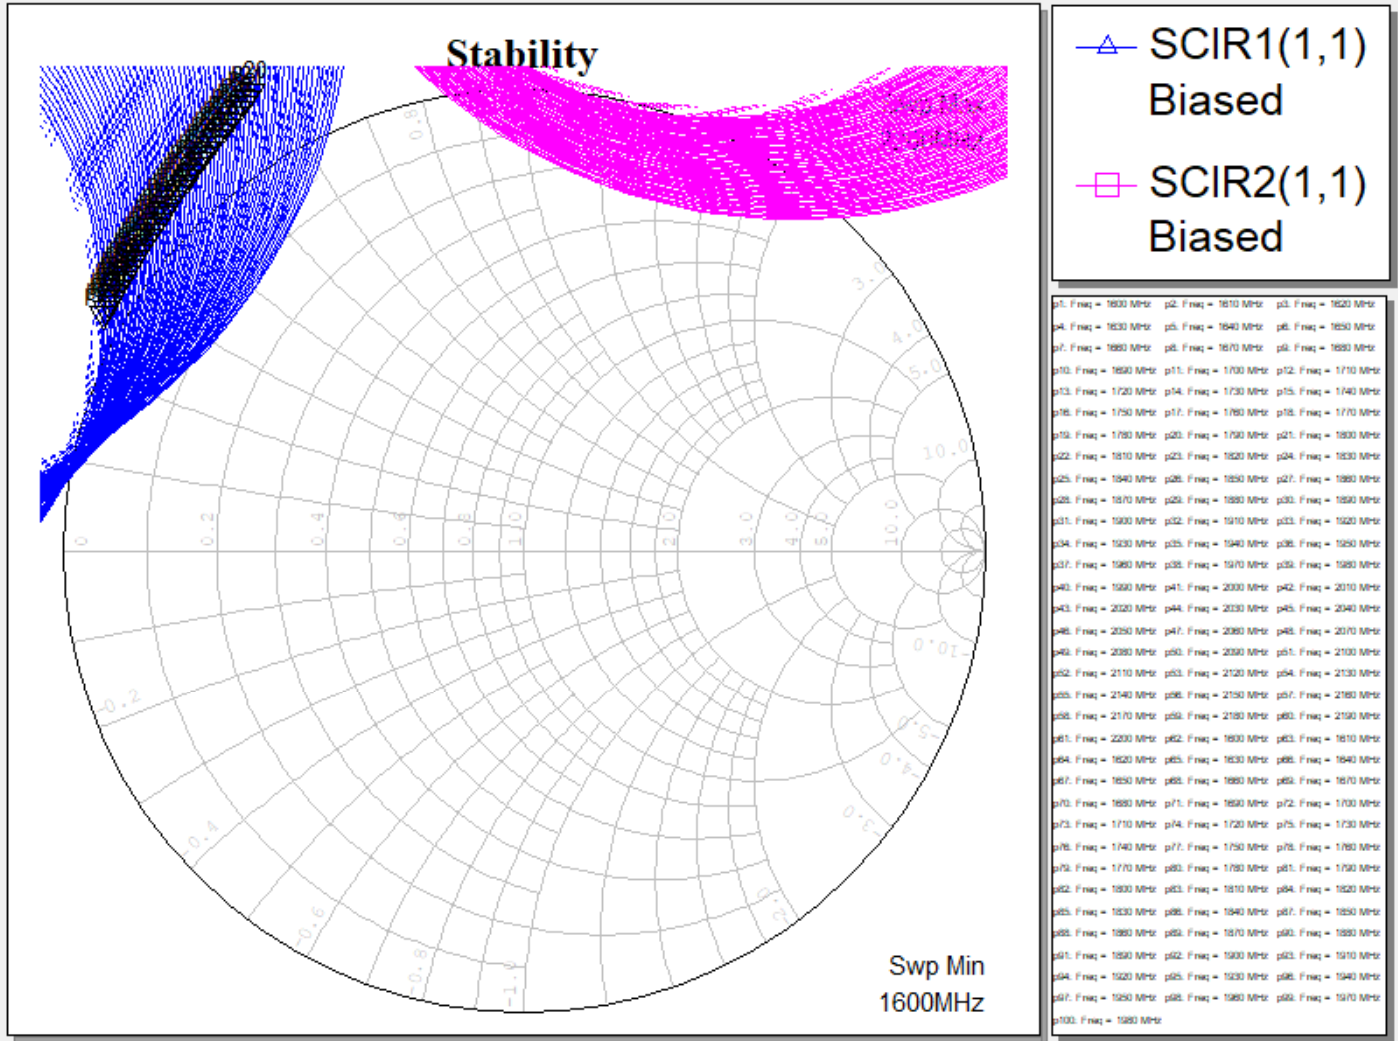
\includegraphics[width=0.45\textwidth]{5 stability circles.png}

    \textbf{Stability before resistive stabilisation.}

    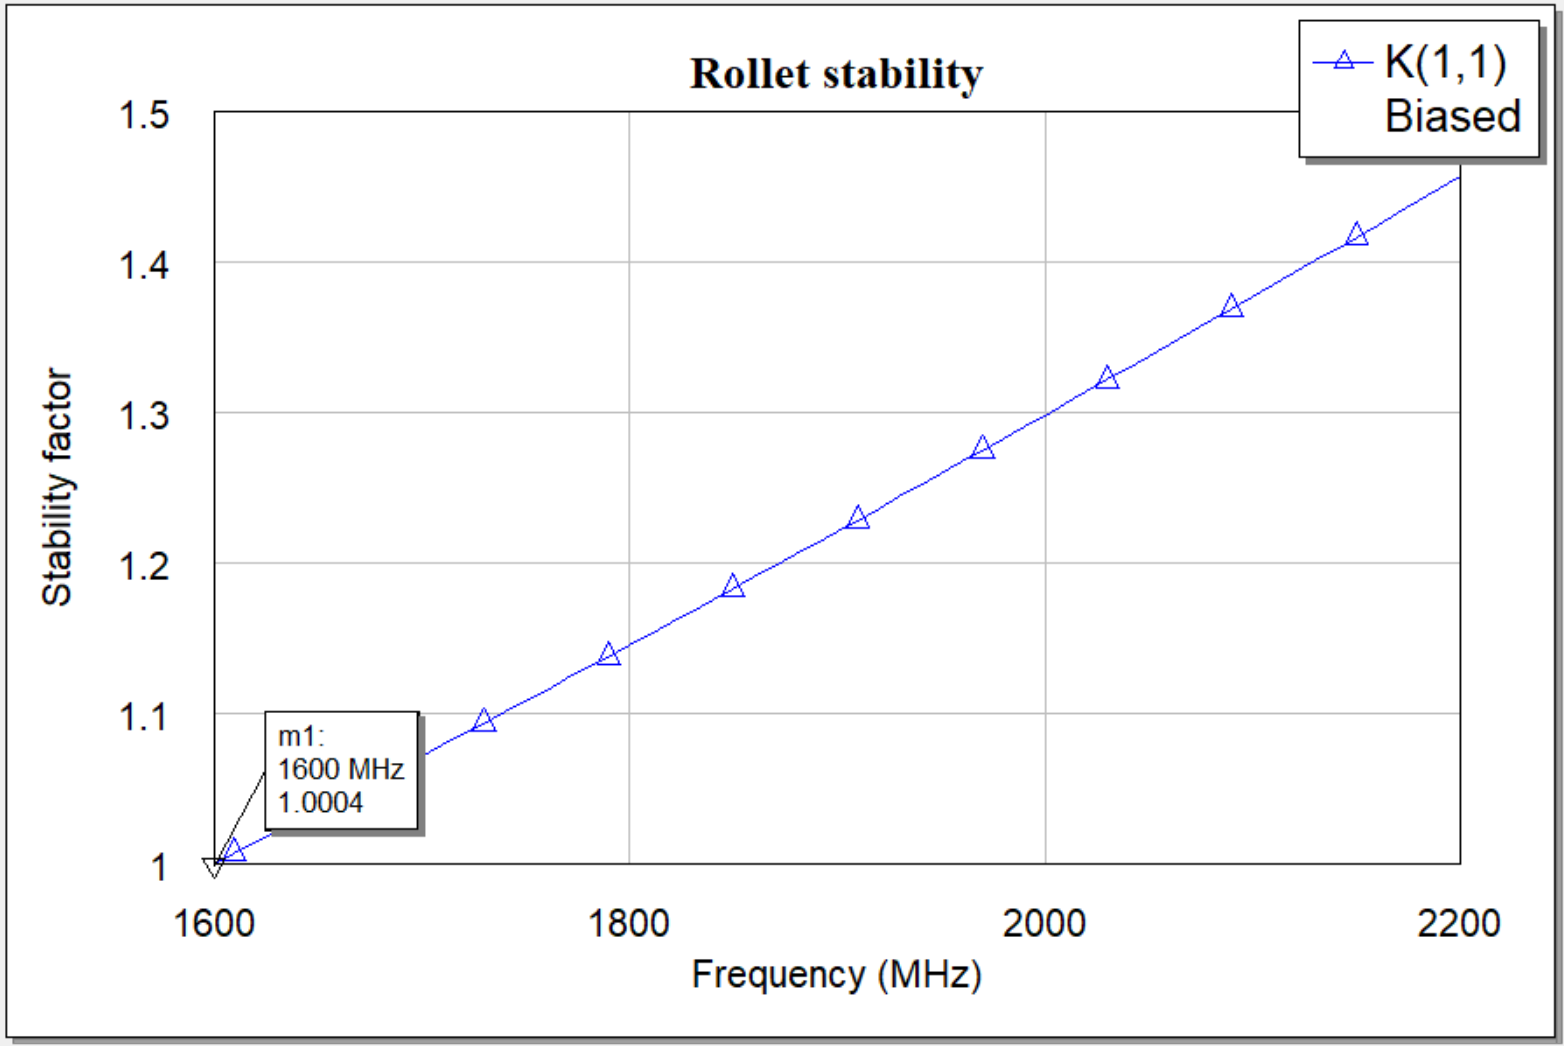
\includegraphics[width=0.5\textwidth]{5 rollet 2.png}
    \quad
    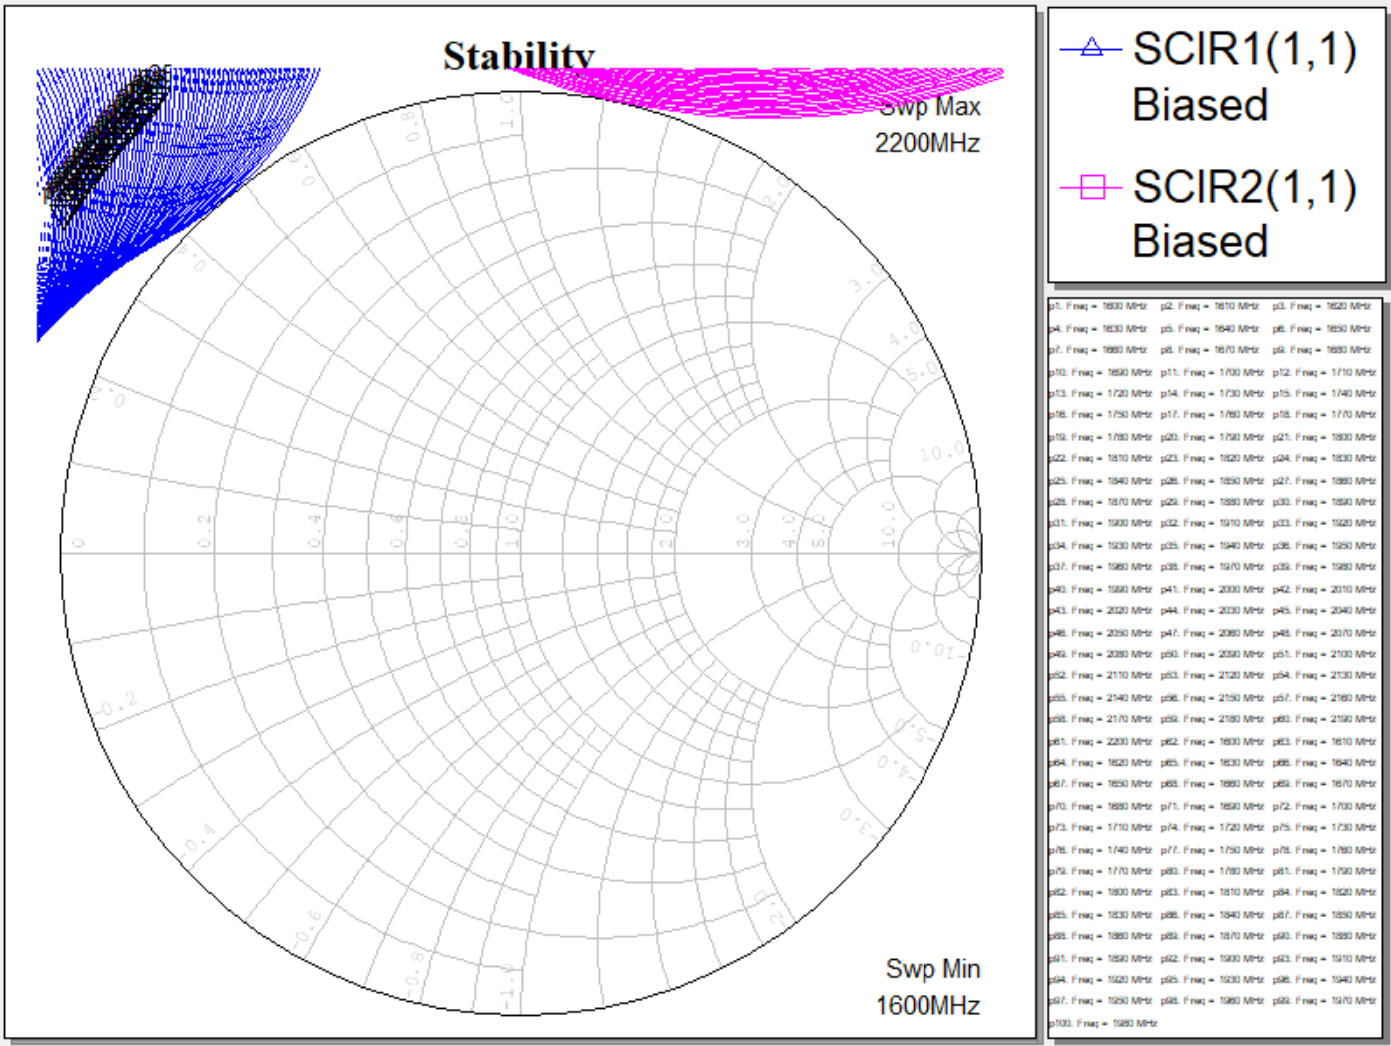
\includegraphics[width=0.45\textwidth]{5 stability circles 2.png}

    \textbf{Stability after stabilisation using 338\,\unit{\ohm} resistor and 20\,\unit{\pico\farad} capacitor.}
\end{center}

\subsection*{(d)}

The system initially has the following S parameters:
\begin{center}
    \begin{tabular}{|c|c|c|c|}
        \hline
        S\textsubscript{11} & S\textsubscript{22} & S\textsubscript{21} & S\textsubscript{12} \\
        \hline  
        $-0.4292 - j0.3964$ & $0.1673 - j0.3998$ & $0.2245 + j1.6266$ & $0.1089 + j0.0617$ \\
        \hline
        $0.5843 \phase{-137.28^{\circ}}$& $0.4334 \phase{-67.296^{\circ}}$ & $1.6420 \phase{82.141^{\circ}}$&$0.1252 \phase{29.523^{\circ}}$  \\
        \hline
    \end{tabular}
\end{center}

This gives the following loads for simultaneous conjugate matching:

$Z_S = 8.6519 + j19.2401, \quad Z_L = 25.3721 + j66.1274$

The following circuit is produced:
\begin{center}
    \frame{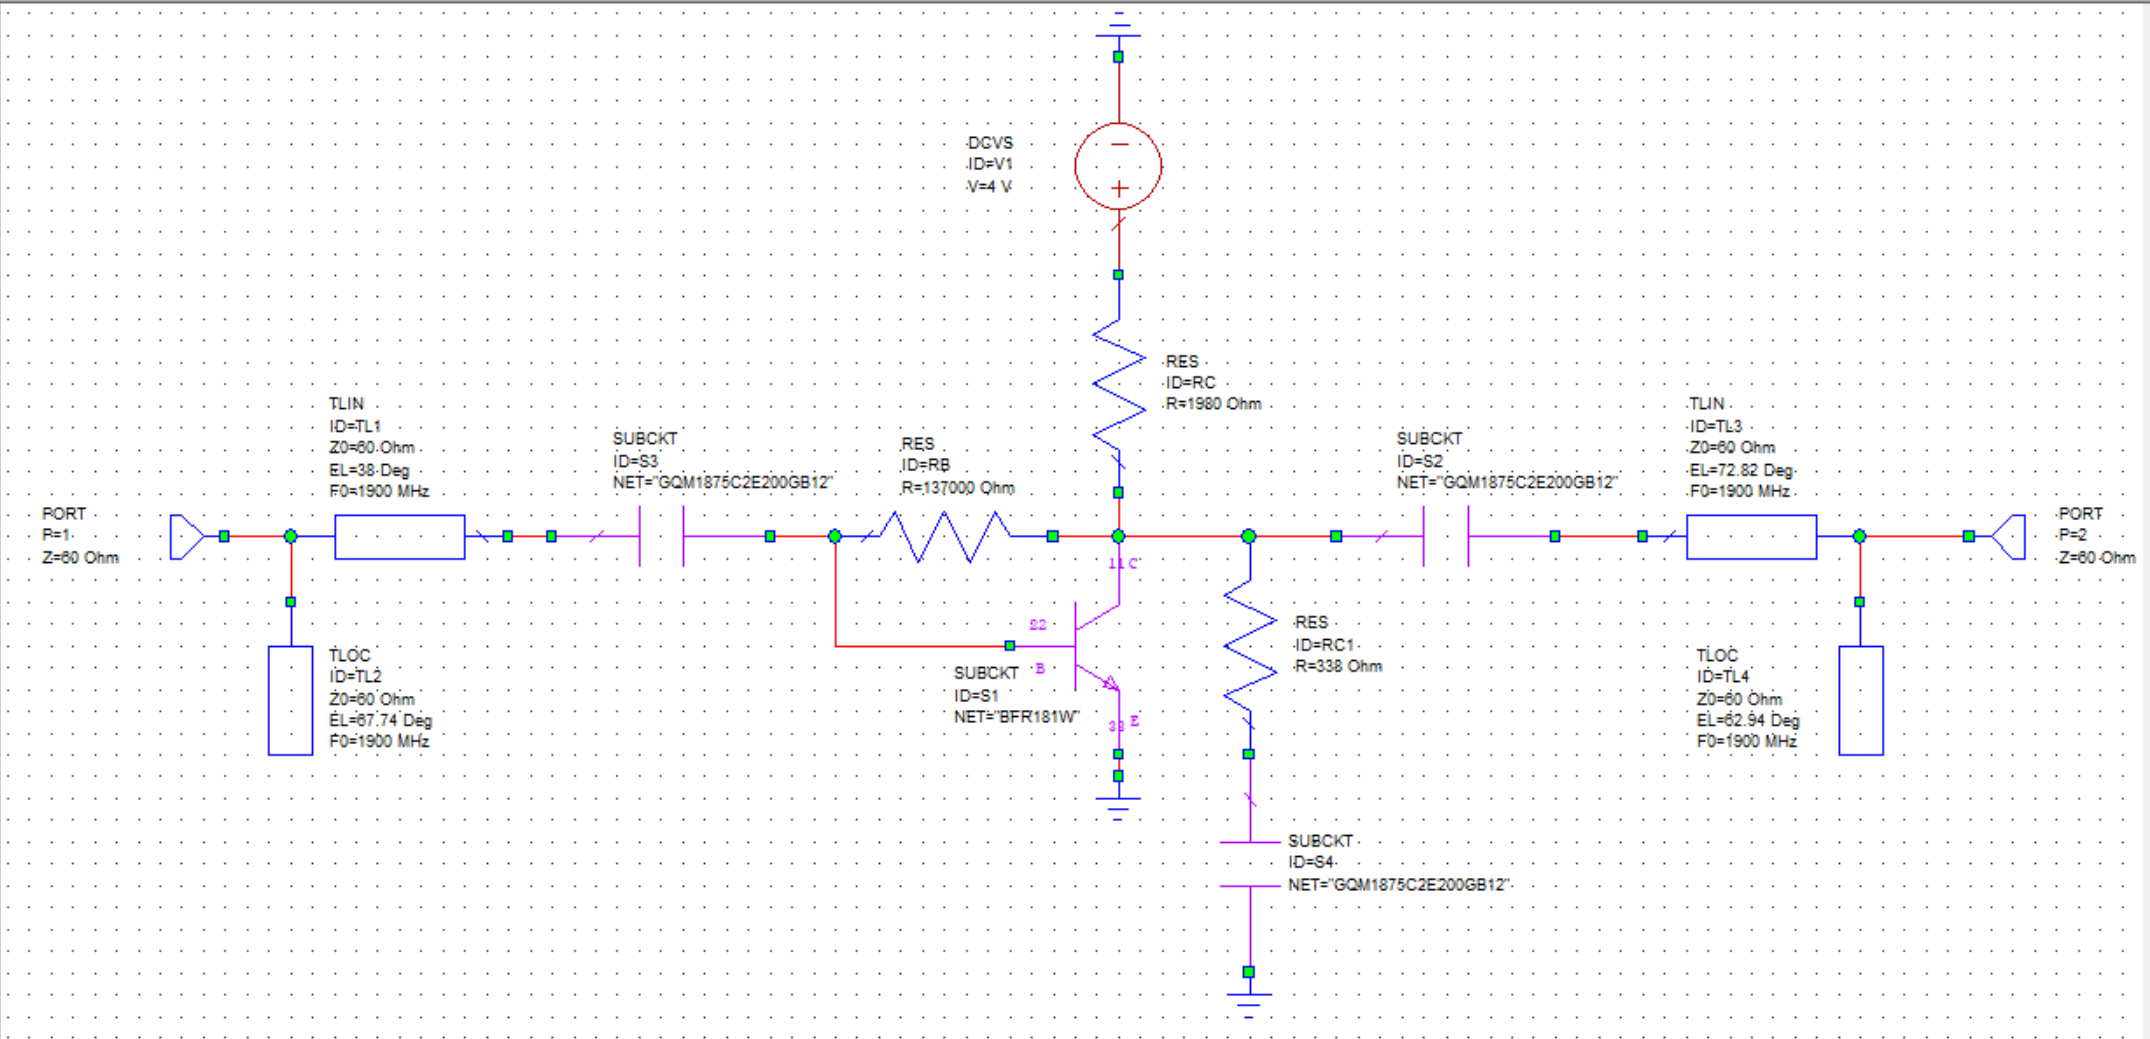
\includegraphics[width=\textwidth]{5 circuit.png}}
\end{center}

Which returns the following parameters:
\begin{center}
    \begin{tabular}{|c|c|c|c|c|}
        \hline
        |S\textsubscript{11}| & |S\textsubscript{22}| & VSWR\textsubscript{input} & VSWR\textsubscript{output} & S\textsubscript{21} \\
        \hline  
        0.01783 & 0.0145 &1.0363 & 1.0294 & 8.3387\,\unit{\decibel}\\
        \hline
    \end{tabular}
\end{center}

The amplifier is overall well matched, with reflection coefficients close to 0 and VSWRs close to 1. 
All parameters appear `better' using simultaneous conjugate matching than with the pre-biased transistor using 
unilateral matching; gain is greater and reflection coefficients are smaller. Values appear very close when 
compared to the simultaneous conjugate matched pre-biased transistor - differences arise from 
slight inaccuracies introduced during the matching process, along with inexact biasing due to using only a single resistor 
from the E192 series for R\textsubscript{B} and R\textsubscript{C}.

\subsection*{(e)}

\begin{center}
    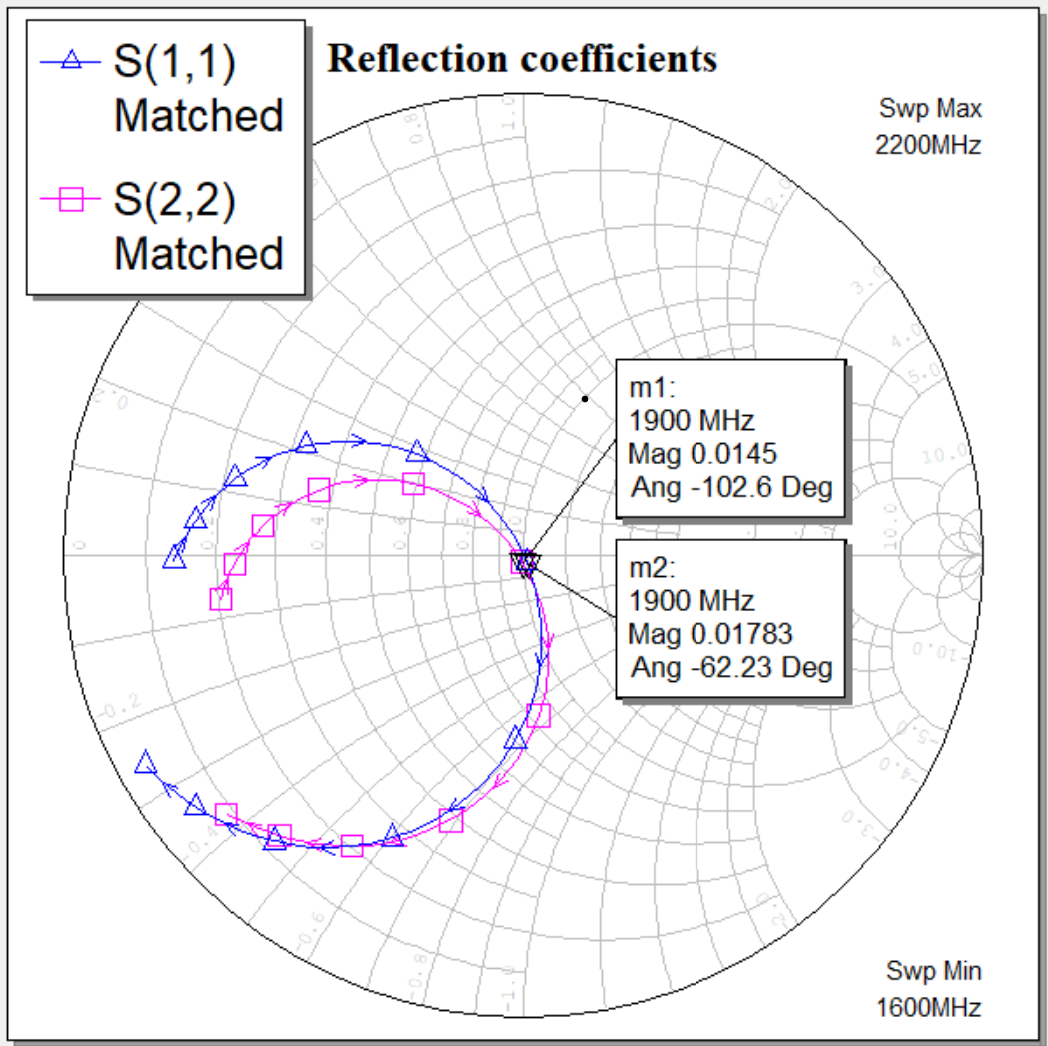
\includegraphics[width=0.8\textwidth]{5 reflection coefficients.png}
    
    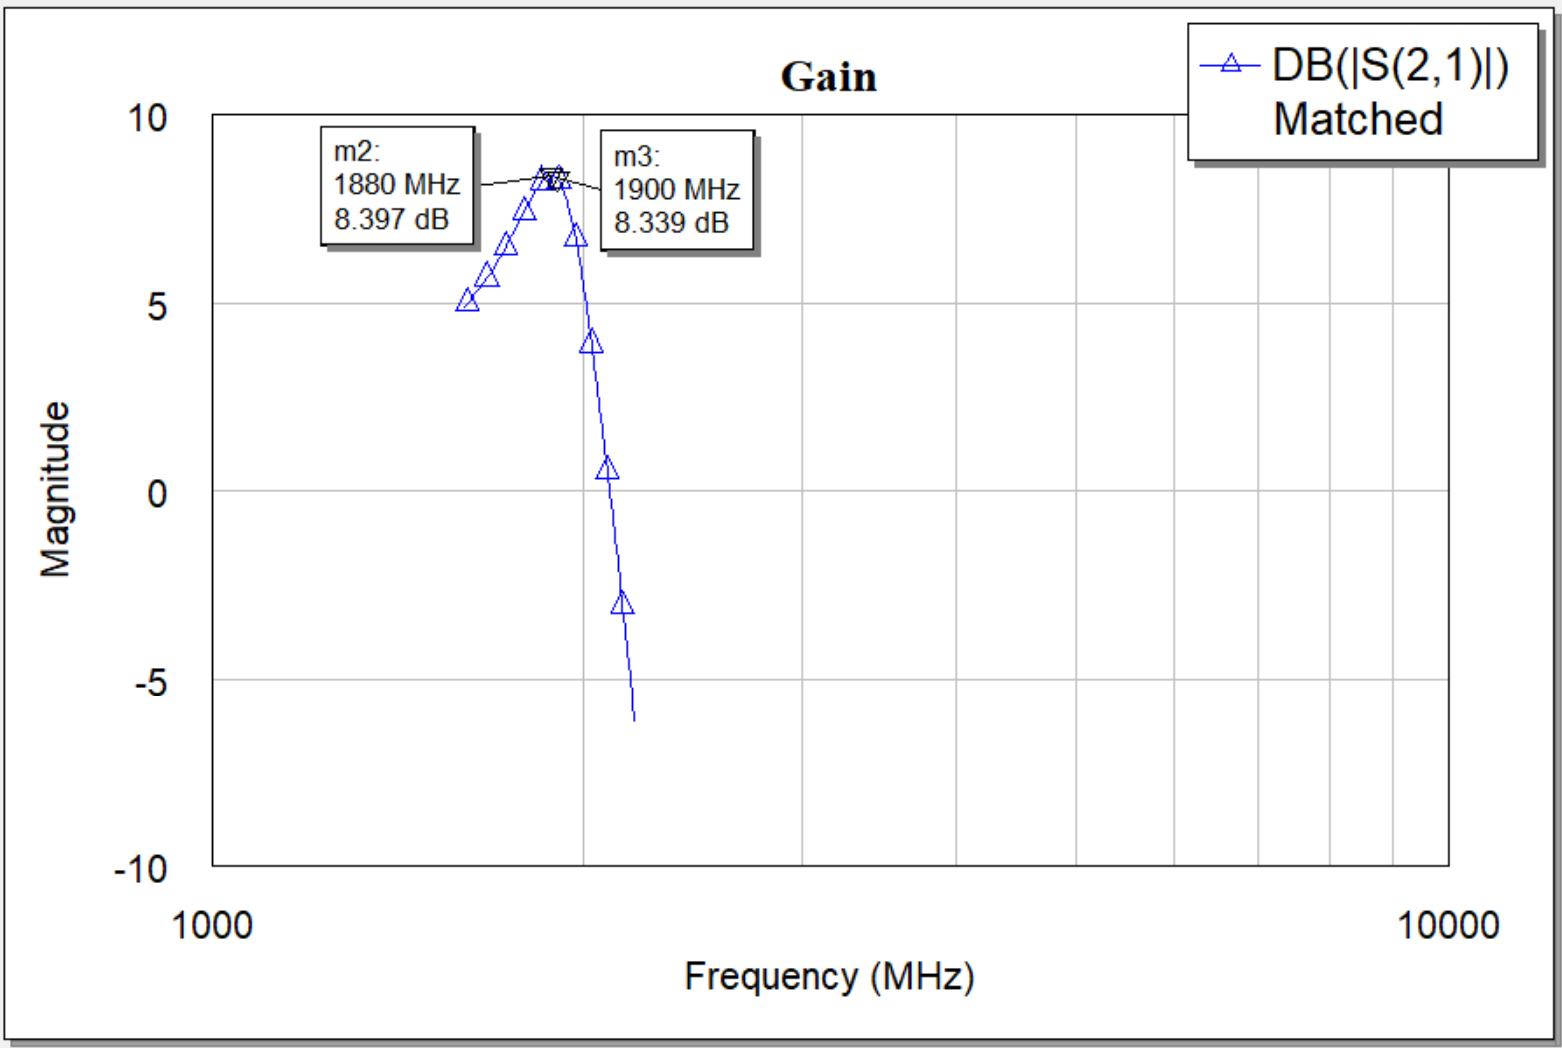
\includegraphics[width=0.8\textwidth]{5 gain.png}
\end{center}

\subsection*{(f)}

$\text{Gain}_{\text{max}} = 8.3409\,\unit{\decibel}$. $\text{Gain}_{\text{design}} = 8.339\,\unit{\decibel}$.
These values are very close, suggesting the designed network approaches the theoretical maximum. 

There ultimately was not a huge difference between the pre-biased transistor model versus the manually biased circuit. 
Some values in the circuit vary somewhat - for example, the stabilisation resistor value was smaller for the non-linear model
due to more sources of impedance introduced into the circuit. The coupling capacitors required for the non-linear transistor 
also would have meant a small variation in the electrical length of the transmission lines (but not more than 5\unit{\degree}).

Both circuits exhibit similar values for maximum gain and gain at the centre frequency. Maximum gain was found at 1.88\,\unit{\giga\hertz}
in both cases. Interestingly, the gain for the non-linear circuit was slightly higher (by $\sim 0.1\,\unit{\decibel}$).

\end{document}

